% Options for packages loaded elsewhere
\PassOptionsToPackage{unicode}{hyperref}
\PassOptionsToPackage{hyphens}{url}
\PassOptionsToPackage{dvipsnames,svgnames,x11names}{xcolor}
%
\documentclass[
]{article}

\usepackage{amsmath,amssymb}
\usepackage{lmodern}
\usepackage{iftex}
\ifPDFTeX
  \usepackage[T1]{fontenc}
  \usepackage[utf8]{inputenc}
  \usepackage{textcomp} % provide euro and other symbols
\else % if luatex or xetex
  \usepackage{unicode-math}
  \defaultfontfeatures{Scale=MatchLowercase}
  \defaultfontfeatures[\rmfamily]{Ligatures=TeX,Scale=1}
\fi
% Use upquote if available, for straight quotes in verbatim environments
\IfFileExists{upquote.sty}{\usepackage{upquote}}{}
\IfFileExists{microtype.sty}{% use microtype if available
  \usepackage[]{microtype}
  \UseMicrotypeSet[protrusion]{basicmath} % disable protrusion for tt fonts
}{}
\makeatletter
\@ifundefined{KOMAClassName}{% if non-KOMA class
  \IfFileExists{parskip.sty}{%
    \usepackage{parskip}
  }{% else
    \setlength{\parindent}{0pt}
    \setlength{\parskip}{6pt plus 2pt minus 1pt}}
}{% if KOMA class
  \KOMAoptions{parskip=half}}
\makeatother
\usepackage{xcolor}
\usepackage[top=30mm,left=25mm,right=25mm,heightrounded]{geometry}
\setlength{\emergencystretch}{3em} % prevent overfull lines
\setcounter{secnumdepth}{-\maxdimen} % remove section numbering
% Make \paragraph and \subparagraph free-standing
\ifx\paragraph\undefined\else
  \let\oldparagraph\paragraph
  \renewcommand{\paragraph}[1]{\oldparagraph{#1}\mbox{}}
\fi
\ifx\subparagraph\undefined\else
  \let\oldsubparagraph\subparagraph
  \renewcommand{\subparagraph}[1]{\oldsubparagraph{#1}\mbox{}}
\fi


\providecommand{\tightlist}{%
  \setlength{\itemsep}{0pt}\setlength{\parskip}{0pt}}\usepackage{longtable,booktabs,array}
\usepackage{calc} % for calculating minipage widths
% Correct order of tables after \paragraph or \subparagraph
\usepackage{etoolbox}
\makeatletter
\patchcmd\longtable{\par}{\if@noskipsec\mbox{}\fi\par}{}{}
\makeatother
% Allow footnotes in longtable head/foot
\IfFileExists{footnotehyper.sty}{\usepackage{footnotehyper}}{\usepackage{footnote}}
\makesavenoteenv{longtable}
\usepackage{graphicx}
\makeatletter
\def\maxwidth{\ifdim\Gin@nat@width>\linewidth\linewidth\else\Gin@nat@width\fi}
\def\maxheight{\ifdim\Gin@nat@height>\textheight\textheight\else\Gin@nat@height\fi}
\makeatother
% Scale images if necessary, so that they will not overflow the page
% margins by default, and it is still possible to overwrite the defaults
% using explicit options in \includegraphics[width, height, ...]{}
\setkeys{Gin}{width=\maxwidth,height=\maxheight,keepaspectratio}
% Set default figure placement to htbp
\makeatletter
\def\fps@figure{htbp}
\makeatother
\newlength{\cslhangindent}
\setlength{\cslhangindent}{1.5em}
\newlength{\csllabelwidth}
\setlength{\csllabelwidth}{3em}
\newlength{\cslentryspacingunit} % times entry-spacing
\setlength{\cslentryspacingunit}{\parskip}
\newenvironment{CSLReferences}[2] % #1 hanging-ident, #2 entry spacing
 {% don't indent paragraphs
  \setlength{\parindent}{0pt}
  % turn on hanging indent if param 1 is 1
  \ifodd #1
  \let\oldpar\par
  \def\par{\hangindent=\cslhangindent\oldpar}
  \fi
  % set entry spacing
  \setlength{\parskip}{#2\cslentryspacingunit}
 }%
 {}
\usepackage{calc}
\newcommand{\CSLBlock}[1]{#1\hfill\break}
\newcommand{\CSLLeftMargin}[1]{\parbox[t]{\csllabelwidth}{#1}}
\newcommand{\CSLRightInline}[1]{\parbox[t]{\linewidth - \csllabelwidth}{#1}\break}
\newcommand{\CSLIndent}[1]{\hspace{\cslhangindent}#1}

\usepackage{booktabs}
\usepackage{longtable}
\usepackage{array}
\usepackage{multirow}
\usepackage{wrapfig}
\usepackage{float}
\usepackage{colortbl}
\usepackage{pdflscape}
\usepackage{tabu}
\usepackage{threeparttable}
\usepackage{threeparttablex}
\usepackage[normalem]{ulem}
\usepackage{makecell}
\usepackage{xcolor}
\usepackage{lineno}
\usepackage[noblocks]{authblk}
\renewcommand*{\Authsep}{, }
\renewcommand*{\Authand}{, }
\renewcommand*{\Authands}{, }
\renewcommand\Affilfont{\small}
\usepackage{setspace}
\nolinenumbers
\makeatletter
\makeatother
\makeatletter
\makeatother
\makeatletter
\@ifpackageloaded{caption}{}{\usepackage{caption}}
\AtBeginDocument{%
\ifdefined\contentsname
  \renewcommand*\contentsname{Table of contents}
\else
  \newcommand\contentsname{Table of contents}
\fi
\ifdefined\listfigurename
  \renewcommand*\listfigurename{List of Figures}
\else
  \newcommand\listfigurename{List of Figures}
\fi
\ifdefined\listtablename
  \renewcommand*\listtablename{List of Tables}
\else
  \newcommand\listtablename{List of Tables}
\fi
\ifdefined\figurename
  \renewcommand*\figurename{Figure}
\else
  \newcommand\figurename{Figure}
\fi
\ifdefined\tablename
  \renewcommand*\tablename{Table}
\else
  \newcommand\tablename{Table}
\fi
}
\@ifpackageloaded{float}{}{\usepackage{float}}
\floatstyle{ruled}
\@ifundefined{c@chapter}{\newfloat{codelisting}{h}{lop}}{\newfloat{codelisting}{h}{lop}[chapter]}
\floatname{codelisting}{Listing}
\newcommand*\listoflistings{\listof{codelisting}{List of Listings}}
\makeatother
\makeatletter
\@ifpackageloaded{caption}{}{\usepackage{caption}}
\@ifpackageloaded{subcaption}{}{\usepackage{subcaption}}
\makeatother
\makeatletter
\@ifpackageloaded{tcolorbox}{}{\usepackage[many]{tcolorbox}}
\makeatother
\makeatletter
\@ifundefined{shadecolor}{\definecolor{shadecolor}{rgb}{.97, .97, .97}}
\makeatother
\makeatletter
\makeatother
\ifLuaTeX
  \usepackage{selnolig}  % disable illegal ligatures
\fi
\IfFileExists{bookmark.sty}{\usepackage{bookmark}}{\usepackage{hyperref}}
\IfFileExists{xurl.sty}{\usepackage{xurl}}{} % add URL line breaks if available
\urlstyle{same} % disable monospaced font for URLs
\hypersetup{
  pdftitle={Multi-material distributed recycling via Material Extrusion: rHDPE and rPET case of study},
  pdfauthor={Catalina Suescun Gonzalez; Fabio A. Cruz Sanchez; Hakim Boudaoud; Cécile Nouvel; Joshuua Pearce},
  pdfkeywords={Multi-material, Recycling, Waste-based, Fused granular
fabrication},
  colorlinks=true,
  linkcolor={Blue},
  filecolor={Maroon},
  citecolor={Blue},
  urlcolor={Blue},
  pdfcreator={LaTeX via pandoc}}

\title{Multi-material distributed recycling via Material Extrusion:
rHDPE and rPET case of study}


\author{Catalina Suescun Gonzalez}
\author{Fabio A. Cruz Sanchez}
\author{Hakim Boudaoud}
\author{Cécile Nouvel}
\author{Joshuua Pearce}

\affil[1]{Université de Lorraine -- ERPI -- F-54000, Nancy, France}
\affil[2]{Université de Lorraine, CNRS, LRGP, F-54000 Nancy, France}
\affil[3]{Western University, Department of Electrical \& Computer
Engineering, Canada, London}


\date{}
\begin{document}
\maketitle
\begin{abstract}
\doublespacing The high volume of plastic waste and the extremely low
recycling rate have created a serious challenge worldwide. Local
distributed recycling coupled with additive manufacturing (DRAM) offers
a solution by economically incentivizing local recycling. One DRAM
technology capable of processing large quantities of plastic waste is
fused granular fabrication (FGF), where solid shredded plastic waste can
be reused directly as 3D printing feedstock. This study presents an
experimental assessment of multi-material recycling printability using
two of the most common thermoplastics in the beverage industry,
polyethylene terephthalate (PET) and high-density polyethylene (HDPE),
and the feasibility of mixing PET and HDPE to be used as a feedstock
material for large-scale 3-D printing. After the material collection,
shredding, and cleaning, the characterization and optimization of
parameters for 3D printing were performed. Results showed the
feasibility of printing a large object from rPET/rHDPE flakes, reducing
the production cost by up to 88\%.
\end{abstract}
\ifdefined\Shaded\renewenvironment{Shaded}{\begin{tcolorbox}[sharp corners, enhanced, breakable, borderline west={3pt}{0pt}{shadecolor}, frame hidden, interior hidden, boxrule=0pt]}{\end{tcolorbox}}\fi

\setstretch{1}
\section*{Acronyms}

\begingroup\fontsize{10}{12}\selectfont

\begin{tabular}{>{}ll}
\toprule
Acronym & Definition\\
\midrule
\textcolor{black}{\textbf{ABS }} & Acrylonitrile Butadiene Styrene  \\
\textcolor{black}{\textbf{AM }} & Additive Manufacturing \\
\textcolor{black}{\textbf{DRAM }} & Distributed recycling via additive manufacturing \\
\textcolor{black}{\textbf{DSC }} & Differential scanning calorimetry  \\
\textcolor{black}{\textbf{FDM }} & Fused deposition modeling \\
\textcolor{black}{\textbf{FFF }} & Fused filament fabrication \\
\textcolor{black}{\textbf{FGF }} & Fused granular fabrication \\
\textcolor{black}{\textbf{FPF }} & Fused particle fabrication \\
\textcolor{black}{\textbf{FTIR }} & Fourier-transform infrared spectroscopy  \\
\textcolor{black}{\textbf{HDPE }} & High-density polyethylene \\
\textcolor{black}{\textbf{MFI }} & Melt flow index \\
\textcolor{black}{\textbf{PC }} & Polycarbonate \\
\textcolor{black}{\textbf{PET }} & Poly(ethylene terephthalate) \\
\textcolor{black}{\textbf{PLA }} & Poly(lactic acid) \\
\textcolor{black}{\textbf{PP }} & Polypropylene  \\
\textcolor{black}{\textbf{PSO }} & Particle swarm optimization \\
\textcolor{black}{\textbf{PS }} & Polystyrene \\
\textcolor{black}{\textbf{SEBS }} & Poly (styrene-block-ethene-co-butene-block-styrene) \\
\textcolor{black}{\textbf{Tg }} & Glass temperature \\
\textcolor{black}{\textbf{pBC }} & Printed Bottle-Cap \\
\textcolor{black}{\textbf{rHDPE }} & Recycled High-density Polyethylene \\
\textcolor{black}{\textbf{rPET90//rHDPE10  }} & Recycled Bottle-Cap (Cristaline bottle shredded without separation) \\
\textcolor{black}{\textbf{rPET }} & Recycled Poly(ethylene) terephthalate \\
\textcolor{black}{\textbf{vPET }} & Virgin or commercial Poly(ethylene terephthalate) \\
\bottomrule
\end{tabular}
\endgroup{}

\setstretch{1.5}

\hypertarget{introduction}{%
\section{Introduction}\label{introduction}}

\linenumbers

The disposal of plastic waste is one of the most challenging current
environmental concerns given its systemic complexity
\protect\hyperlink{ref-evode2021}{{[}1{]}}. The mass of micro- / meso-
plastics in the oceans is expected to exceed the mass of the global
stock of fish by 2050 \protect\hyperlink{ref-macarthur2017}{{[}2{]}}.
More critically, the global annual plastic production is expected to
reach 1100 metric tons by the same year
\protect\hyperlink{ref-geyer2020}{{[}3{]}}. Societal awareness of
plastic recycling has received substantial attention from scientists,
policymakers, and the general public
\protect\hyperlink{ref-soares2021}{{[}4{]}}. Unfortunately, the
statistical analysis of the centralized recycling process proves that it
has been largely ineffective
\protect\hyperlink{ref-Siltaloppi2021}{{[}5{]}} with only 9\% of the
plastic produced since 1950 being recycled from the total stock
\protect\hyperlink{ref-Geyer2017}{{[}6{]}}. Therefore, it remains an
open challenge to identify alternatives to valorize discarded plastic
material.

Distributed recycling and additive manufacturing (DRAM) is an innovative
technical approach to recycling plastic waste
\protect\hyperlink{ref-cruzsanchez2020}{{[}7{]}},
\protect\hyperlink{ref-dertinger2020}{{[}8{]}}. DRAM was initially
implemented using recyclebots, which are waste plastic extruders that
produce filament for conventional fused filament-based 3-D printers
\protect\hyperlink{ref-baechler2013}{{[}9{]}}--\protect\hyperlink{ref-woern2018}{{[}11{]}}.
Previous studies have shown that distributed recycling aligns with the
circular economy paradigm \protect\hyperlink{ref-Ford2016}{{[}12{]}},
\protect\hyperlink{ref-Despeisse2016}{{[}13{]}}. This approach allows
consumers to directly recycle their own waste into consumer products
using open-source designs, ranging from toys for children
\protect\hyperlink{ref-Petersen2017}{{[}14{]}} to adaptive aids for
individuals with arthritis \protect\hyperlink{ref-gallup2018}{{[}15{]}}.
Distributed manufacturing is now widely adopted
\protect\hyperlink{ref-pearce2022}{{[}16{]}}. In this way, DRAM-based
recycling operates within a closed-loop supply chain network
\protect\hyperlink{ref-santander2020}{{[}17{]}}. The primary goal of
this type of recycling is to reduce the environmental impact by
minimizing the transportation from the waste source to recycling
facilities \protect\hyperlink{ref-kreiger2014}{{[}18{]}}. In that sense,
it aims to propose innovative closed-loop strategies that utilize waste
materials as raw resources \protect\hyperlink{ref-romani2021}{{[}19{]}}.

Fused filament fabrication (FFF, which is also known as Fused Deposition
Modelling --FDM©-) is the most widespread and established
extrusion-based AM technology. It has gained popularity due to the
open-source proliferation from the self-replicating rapid prototyper
(RepRap) project
\protect\hyperlink{ref-jones2011}{{[}20{]}}--\protect\hyperlink{ref-bowyer2014}{{[}22{]}}.
FFF is favored for its simplicity, versatility, low cost, and ability to
construct complex geometric objects in the industrial and prosumer
domains \protect\hyperlink{ref-romani2021}{{[}19{]}}. Indeed, the
open-source approach for 3-D printing has facilitated significant
advancements in manufacturing and prototyping adding value to the
recycled material \protect\hyperlink{ref-cruzsanchez2020}{{[}7{]}}.
Efforts are being made to identify sustainable feedstocks for 3-D
printing \protect\hyperlink{ref-Pakkanen2017}{{[}24{]}}. Several studies
have expanded the range of recycled filament materials including PLA
\protect\hyperlink{ref-cruzsanchez2017}{{[}25{]}},
\protect\hyperlink{ref-anderson2017}{{[}26{]}}, ABS
\protect\hyperlink{ref-mohammed2017a}{{[}27{]}},
\protect\hyperlink{ref-mohammed2017}{{[}28{]}}, PET
\protect\hyperlink{ref-zander2018}{{[}29{]}},
\protect\hyperlink{ref-vaucher2022}{{[}30{]}}, HDPE
\protect\hyperlink{ref-baechler2013}{{[}9{]}},
\protect\hyperlink{ref-mohammed2017a}{{[}27{]}},
\protect\hyperlink{ref-chong2017}{{[}31{]}}, and PC
\protect\hyperlink{ref-gaikwad2018}{{[}32{]}}. In fact,
\protect\hyperlink{ref-kreiger2014}{{[}18{]}} conducted a comparative
life cycle assessment in a low-density population case study in Michigan
(USA) and estimated that a distributed approach could save approximately
100 billion MJ of energy per year from the recycling of 984 million
pounds of HDPE. There is substantial evidence that DRAM can contribute
to reducing energy consumption and greenhouse emissions in manufacturing
processes.

Most DRAM studies have used mono-materials for the fabrication of
feedstock for FFF. There are, however, several examples of mixed
materials including wood waste and recycled plastic
\protect\hyperlink{ref-pringle2018}{{[}33{]}},
\protect\hyperlink{ref-loschke2019}{{[}34{]}} and textile fibers and
recycled plastic \protect\hyperlink{ref-carrete2021}{{[}35{]}}.
Recently, \protect\hyperlink{ref-Zander2019}{{[}36{]}} reported the
manufacturing of composite filament from recycled PET/PP and PS/PP
blending through a compatibilizer copolymer such as SEBS. Their results
revealed the technical printability of polypropylene blend composite
filaments from a thermo-mechanical characterization perspective.
Increasing the performance window of blending materials by
compatibilization which could be a relevant path for recycling plastics
at a local level and in isolated areas contexts (e.g.~during
humanitarian crises
\protect\hyperlink{ref-savonen2018}{{[}37{]}}--\protect\hyperlink{ref-lipsky2019}{{[}39{]}},
supply chain disruptions \protect\hyperlink{ref-novak2020}{{[}40{]}},
\protect\hyperlink{ref-choong2020}{{[}41{]}},
\protect\hyperlink{ref-salmi2020}{{[}42{]}},
\protect\hyperlink{ref-attaran2020}{{[}43{]}} and/or isolated off-grid
situations using solar-powered 3-D printers
\protect\hyperlink{ref-king2014}{{[}44{]}}--\protect\hyperlink{ref-Mohammed2018}{{[}47{]}}).
Likewise, \protect\hyperlink{ref-vaucher2022}{{[}30{]}} studied the
evaluation of the microstructure, mechanical performance, and printing
quality of filaments made from rPET and rHDPE varying the wt\% of HDPE
material from 0 to 10\%. They confirmed the increase in Young's modulus
from 1.7 GPa of the pure PET to 2.1 GPa for all the HDPE concentrations.
Additionally, the maximum stress of the bends was augmented with high
HDPE concentrations. Values were lower than virgin PET filament, yet
similar to commercial recycle ones. The addition of rHDPE at higher
levels, however, helped to meet the brittle-ductile transition in 15\%
despite the low interfacial tension of both polymers, allowing the
printing of quality parts.

While former studies have proven successful in FFF, a new approach to
DRAM is fused granular fabrication (FGF) or fused particle fabrication
(FPF), where the material-extrusion AM systems print directly from
pellets, granules, flakes, shreds or grinder material
\protect\hyperlink{ref-woern2018}{{[}11{]}},
\protect\hyperlink{ref-fontana2022}{{[}48{]}}. In the context of
recycling, this could reduce the number of melt/extrusion cycles that
degrade the material needed in the filament fabrication process
\protect\hyperlink{ref-cruzsanchez2017}{{[}25{]}}. The FGF technique
opens up the potential to use recycled materials as well as print
large-scale objects either with a conventional cartesian 3-D printer
\protect\hyperlink{ref-woern2018}{{[}11{]}}, delta 3-D printer
\protect\hyperlink{ref-grassi2019}{{[}49{]}} or hangprinter
\protect\hyperlink{ref-petsiuk2022}{{[}50{]}},
\protect\hyperlink{ref-rattan2023}{{[}51{]}}. Research groups have
corroborated that plastic waste can be used as feedstock materials for
FGF/FPF. \protect\hyperlink{ref-alexandre2020}{{[}52{]}} assessed the
technical and economical dimensions of virgin and shredded PLA printed
in a self-modified FGF machine and compared it with FFF. The
investigation showed that the use of FGF reduced printing costs, time
and its mechanical performance was comparable to that obtained using the
traditional FFF technique. Likewise,
\protect\hyperlink{ref-woern2018}{{[}11{]}} found comparable properties
between PLA, ABS, PP, and PET recycled and virgin materials. Later
publications demonstrated the technical and economic feasibility through
the printing of complex objects validating the possibility of recycling
plastic with FGF in both conventional and common FFF materials
\protect\hyperlink{ref-byard2019}{{[}53{]}}, but also recycling PC
\protect\hyperlink{ref-reich2019b}{{[}54{]}} and rPET
\protect\hyperlink{ref-little2020}{{[}55{]}}. Few researchers, however,
have addressed the problem of directly printing recycled
multi-materials, which might be a key step forward needed to facilitate
the ease of sorting and recycling post-consumer plastic waste materials.

This study explores the potential of direct 3-D printing of two
immiscible polymers commonly used in the beverage sector through a
distributed recycling process for its easy implementation operation at
the local level. To demonstrate the feasibility of the process, the most
commonly used plastic for bottled water in France, which consists of
roughly 90\% PET (body of the bottle) and 10\% HDPE (cap) now referred
to as \emph{rPET90//rHDPE10}, is used as a test material. The
experimental process of collection, characterization, and printing of
the recycled material is described, and the results are discussed in the
context of widespread DRAM adoption at the community-based level.

\hypertarget{materials-and-methods}{%
\section{Materials and Methods}\label{materials-and-methods}}

The methodology presented in Figure~\ref{fig-1} outlines the approach
adopted to develop the study. The three stages, namely \emph{Material
obtention}, \emph{Printing process}, and \emph{Evaluation} were
thoroughly studied to control the major process steps and the technical
characterization methods. In the following subsections, each step is
explained.

\begin{figure}

{\centering \includegraphics[width=0.9\textwidth,height=\textheight]{figures/Fig_1_framework.png}

}

\caption{\label{fig-1}Global framework of the study}

\end{figure}

\hypertarget{raw-material-obtention}{%
\subsection{Raw material obtention}\label{raw-material-obtention}}

The goal of the material stage is to collect and prepare post-consumer
plastic sources. In this study, water bottles coming from the French
brand Cristaline\textsuperscript{\textcopyright} were used as feedstock.
The process steps used are shown in Figure~\ref{fig-fig1} a/b.
Post-consumer bottles were collected from receptacles placed in
partnership schools in Lorraine, France. To convert the complete water
bottles including their caps into 3DP feedstock material, the labels
were removed before shredding in a cutting mill (Retsch MS300) using a 3
\(mm\) grid. After shredding, the obtained flakes were sifted with a 1.5
\(mm\), 3 \(mm\), and 5 \(mm\) sifters for further analysis. Next, the
flakes were cleaned with hot water in an ultrasonic machine at 60°C for
1 hour to remove contaminants. Lastly, they were dried in a conventional
oven overnight at 80°C
\protect\hyperlink{ref-vandevoorde2022}{{[}56{]}},
\protect\hyperlink{ref-taghavi2018}{{[}57{]}} to avoid degradation of
the material. Washing conditions were the same for all the samples;
therefore, the effect of contaminants was not considered. The resultant
material is shown in Fig 2.c.

\begin{figure}

{\centering 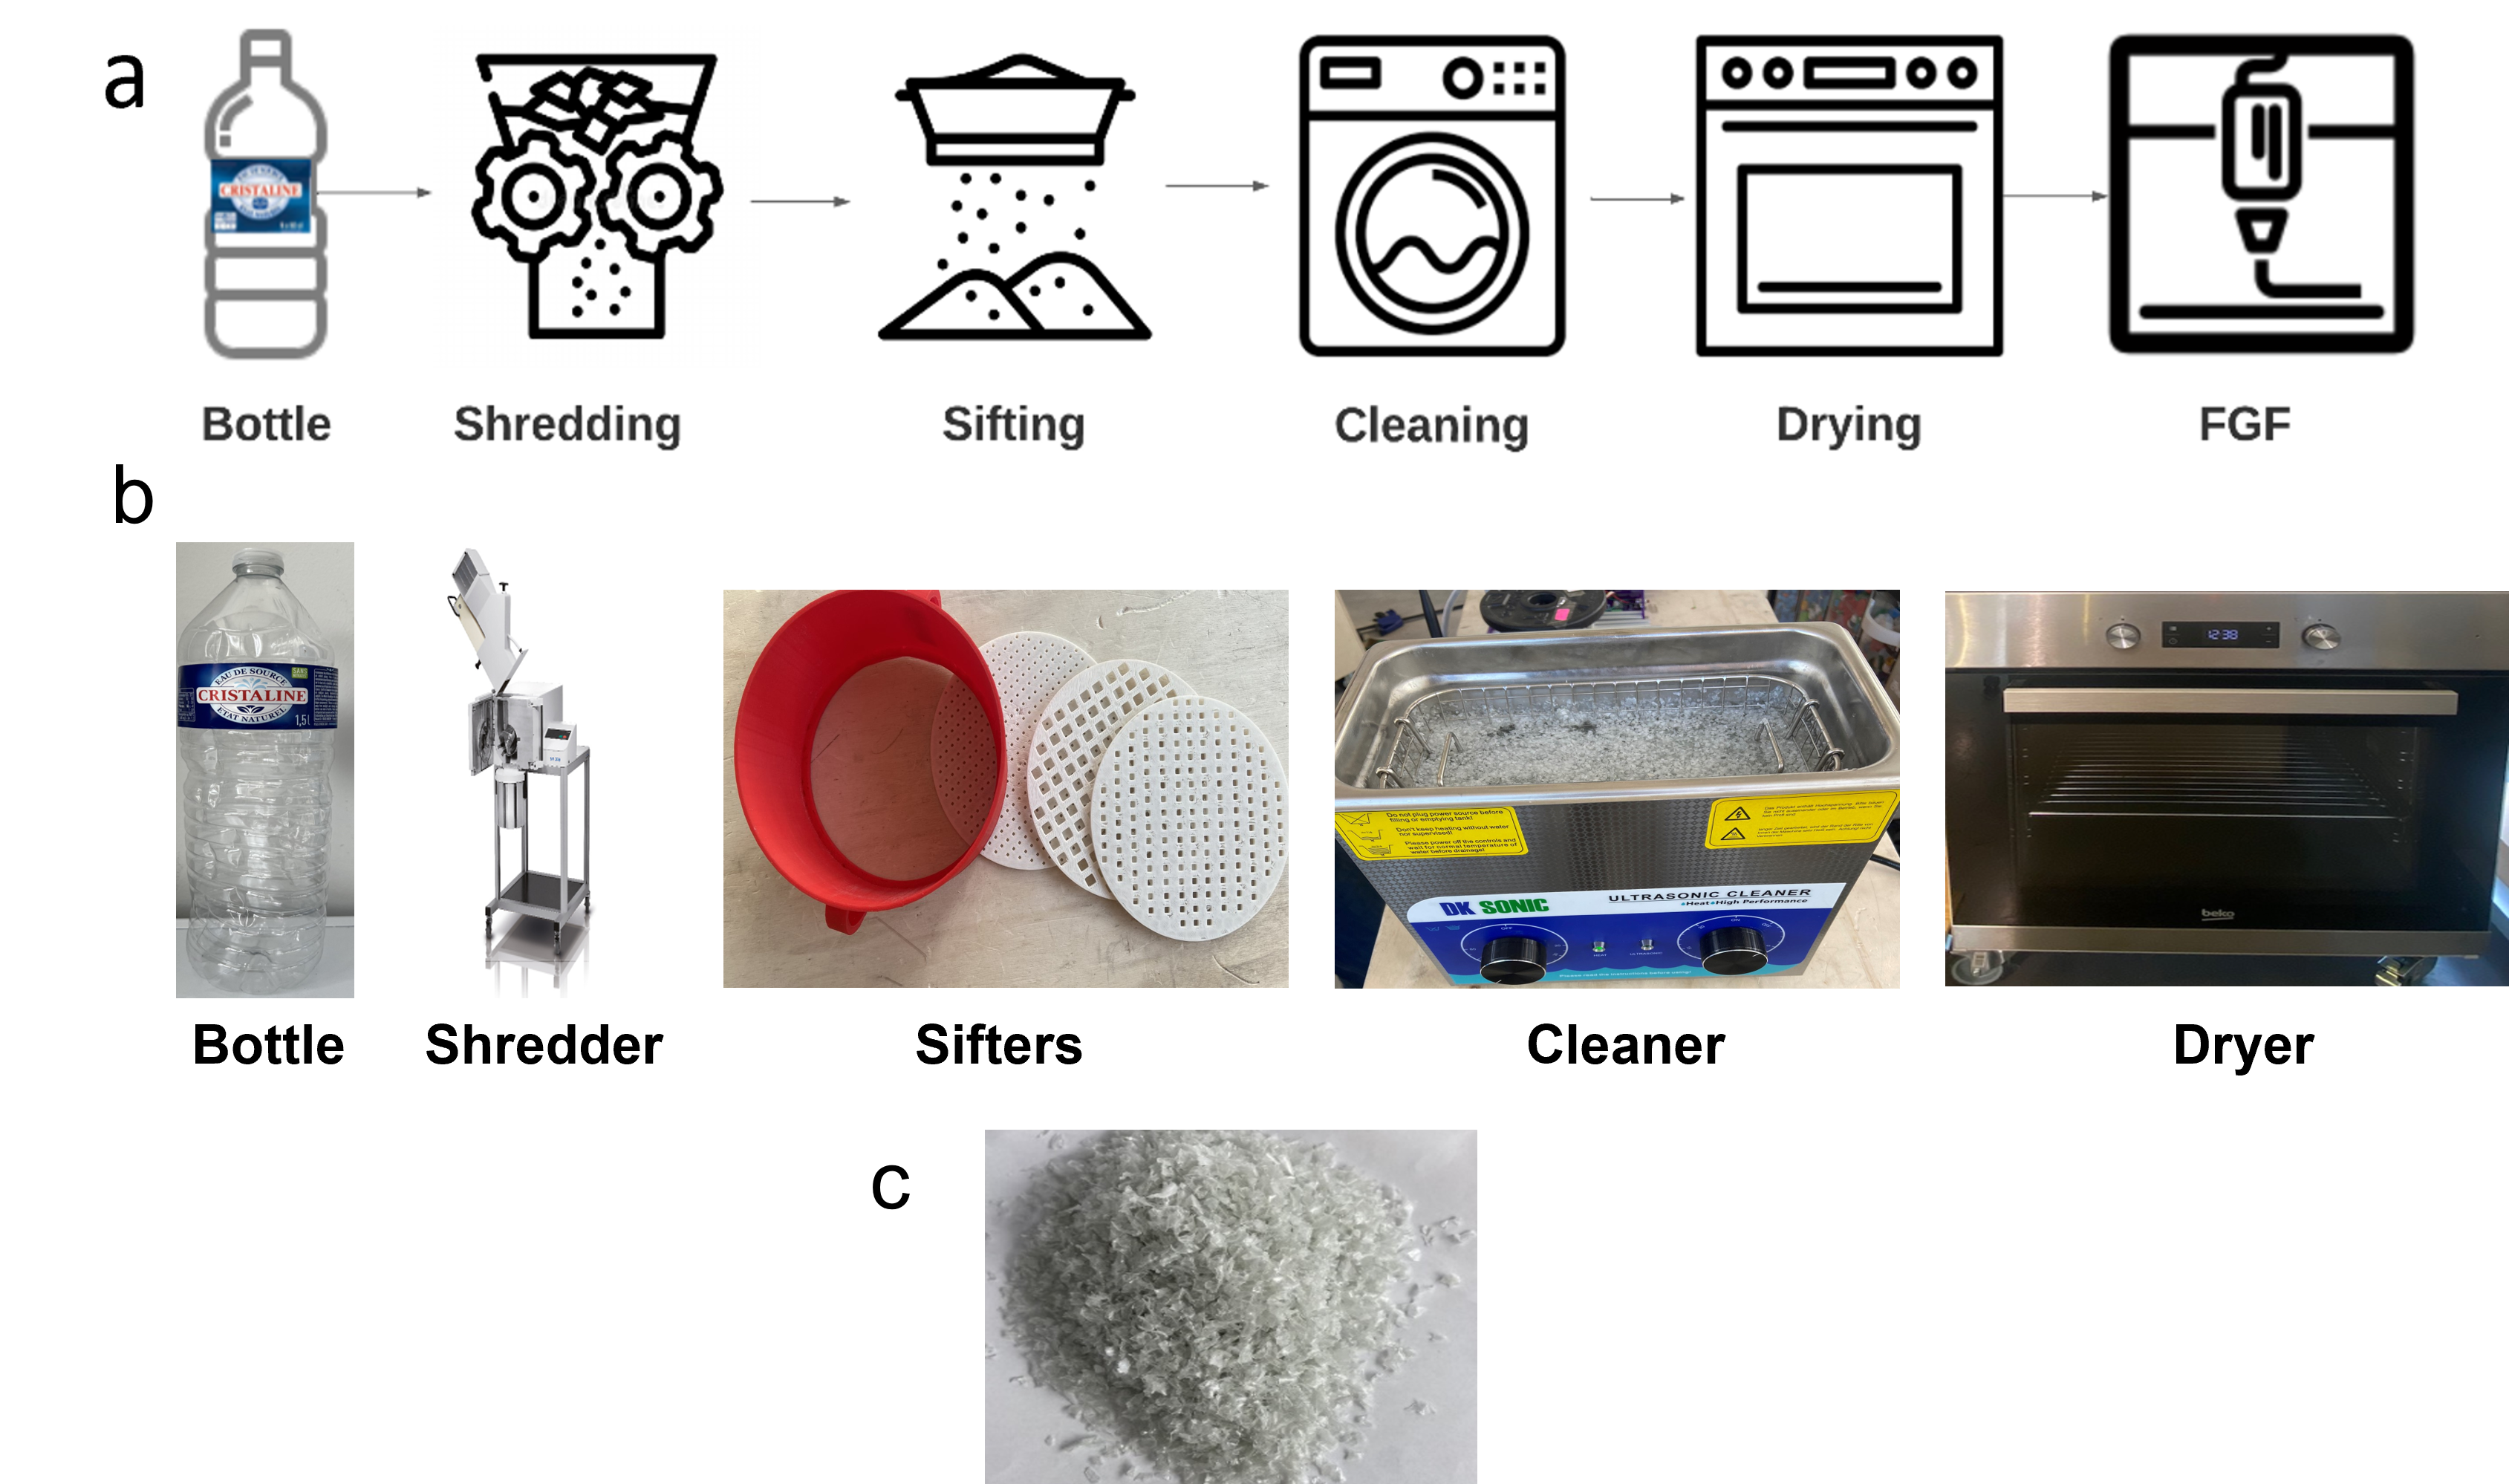
\includegraphics{figures/Fig_2.png}

}

\caption{\label{fig-fig1}Process steps to prepare the collected
material}

\end{figure}

The material composition was calculated as a function of the mass of the
bottles and caps separately. The percentage (\%) of bottle-cap was found
to be \textasciitilde90\%rPET (bottle) and \textasciitilde10\% rHDPE
(cap). The complete bottle was shredded without separation of both
materials thus this percentage is constant for all the samples.

\hypertarget{material-preparation-and-characterization}{%
\subsection{Material preparation and
characterization}\label{material-preparation-and-characterization}}

\hypertarget{material-particle-size-analysis--granulometry-}{%
\subsubsection{Material particle size analysis
-Granulometry-}\label{material-particle-size-analysis--granulometry-}}

In order to ensure the particle size suitable for printing, the
granulate particles were characterized using the open-source ImageJ
software \protect\hyperlink{ref-imagej2023}{{[}58{]}}. The size
characteristics of the particles were evaluated in four different
samples: vPET (used as a reference) and the raw material sifted into
three different sizes: \(1.5~mm\), \(3~mm\), and \(5~mm\).

\hypertarget{fourier-transform-infrared-spectroscopy-ftir-}{%
\subsubsection{Fourier-transform infrared spectroscopy
--FTIR-}\label{fourier-transform-infrared-spectroscopy-ftir-}}

FTIR spectroscopy was conducted to determine the composition of the
bottle and identify any impurities, plasticizers, or additives. The
analysis involving testing separate samples of rPET and rHDPE.
Additionally, a printed sample of both materials was examined to
identify any potential chemical bonding. Each sample was measured at two
different points, with three measurements taken at each point. The
resulting curves were then normalized and analyzed using Origin Pro 8.
The Fourier transform infrared spectra were recorded in the range of
\(4000~cm^{-1}\) to \(375~cm^{-1}\) with a resolution of \(4~cm^{-1}\)
using a Bruker IFS 66V spectrophotometer.

\hypertarget{differential-scanning-calorimetry-dsc-}{%
\subsubsection{Differential scanning calorimetry
--DSC-}\label{differential-scanning-calorimetry-dsc-}}

Differential scanning calorimetry analysis was performed using a DSC-1
Mettler Toledo with STARe software operating under nitrogen atmosphere
at heating rate and cooling rate of \(10~°C/min\). The samples
investigated were rPET, rHDPE, and rPET90//rHDPE10. Three cycles were
conducted: the first involved heating from 20°C to 270°C, cooling to
20°C and reheating to 270°C. The rHDPE sample was analyzed using similar
cycles but with the maximum temperature set at 250°C and the blend was
tested at temperatures ranging from -20 to 270°C. The glass transition
temperature (Tg) of rPET was determined during the first heating cycle,
while the Tg of rPET90//rHDPE10 was determined during the second heating
cycle, along with the melting point of all materials. The
crystallization temperature (Tc) was determined during the cooling cycle
for each material. The degree of crystallinity (Xc) was calculated from
the second cycle for recycled materials and the first cycle for the
blend, as expressed in equation (1)
\protect\hyperlink{ref-taghavi2018}{{[}57{]}},
\protect\hyperlink{ref-pan2020}{{[}59{]}}:

\begin{equation}\protect\hypertarget{eq-dsc}{}{
X_{c}(\%) = \frac{\Delta H_{m}}{w \cdot \Delta H_{m}^\circ}
}\label{eq-dsc}\end{equation}

Where, \(\Delta H_{m}\) is the latent heat of melt, \(w\) is the weight
percentage of polymer in the blend, and \(\Delta H_{m}^\circ\) is the
reference heat of 100\% crystalline PET (\(140~J/g\)) and HDPE
(\(293~J/g\)), respectively, provided in the literature
\protect\hyperlink{ref-pan2020}{{[}59{]}},
\protect\hyperlink{ref-kratofil2006}{{[}60{]}}.

\hypertarget{melt-flow-index-mfi-}{%
\subsubsection{Melt Flow Index --MFI-}\label{melt-flow-index-mfi-}}

The melt-flow index (MFI) of rPET90//rHDPE10 flakes was determined using
an Instron CEAST MF20. The analysis was performed using three samples of
\textasciitilde5 g at a temperature of 255 °C with a 2.16 kg weight
following the ASTM D1238 standard. The process was repeated three times.
The average value of the three results was reported in units of
\(gr/10 \times min\).

\hypertarget{density}{%
\subsubsection{Density}\label{density}}

The material's density was calculated as follows: first, the volume was
found by measuring the dimensions of a solid \(50x50x50~mm\) cubic
geometry fabricated by injecting rPET90//rHDPE10 flakes into a square
mold with a known volume using an open-source desktop injection
machine(Holipress, Holimaker, France). Then, the model was weighed, and
the mass was obtained. Finally, the density was calculated as expressed
in Equation~\ref{eq-density}. To ensure the accuracy of the test it was
performed twice and the average value was reported in \(g/cm^{3}\).

\begin{equation}\protect\hypertarget{eq-density}{}{
\rho = V/m    \qquad \left[ \frac{g}{cm^{3}} \right]
}\label{eq-density}\end{equation}

Where, \(\rho\) is the density, \(V\) is the volume, and \(m\) the mass.

Afterwards, experimental results were compared with the theoretical
blend density which could be calculated by
Equation~\ref{eq-density_theory}.

\begin{equation}\protect\hypertarget{eq-density_theory}{}{
\rho_{12}= \frac{1}{\frac{W_{1}}{\rho_{2}} + \frac{W_{2}}{\rho_{2}}} \qquad \left[ \frac{g}{cm^{3}} \right]                                               
}\label{eq-density_theory}\end{equation}

Where, \(\rho_{12}\) is the density of the blend, \(W_{1}\) and
\(W_{2}\), the weight fractions of each polymer, \(\rho_{1}\) and
\(\rho_{2}\), the theoretical density of each polymer for PET
(\(~1.38~g/cm^{3}\)) and HDPE 0.93 to 0.97 \(g/cm^{3}\)
\protect\hyperlink{ref-jonathanguidigo12017}{{[}61{]}}.

\hypertarget{printing-process}{%
\subsection{Printing process}\label{printing-process}}

\hypertarget{establishing-optimal-parameters}{%
\subsubsection{Establishing optimal
parameters}\label{establishing-optimal-parameters}}

Establishing the optimal combinations of parameters is essential for
improve the quality and mechanical properties of printed parts
\protect\hyperlink{ref-jaisinghsheoran2020}{{[}62{]}}. According to
\protect\hyperlink{ref-oberloier2022}{{[}63{]}}, particle swarm
optimization (PSO) is an accurate and time-effective method for achiving
this goal. To optimize the 3-D printing parameters for the
rPET90//rHDPE10 material in the GigabotX we utilized the open-source PSO
Experimenter platform which is available for Linux. The methodology
developed by \protect\hyperlink{ref-oberloier2022}{{[}63{]}} was
followed during the optimization. For benchmarking purposes, three
artifacts were printed: a line, a plane, and a cube. These artifacts
were modeled in CAD software Onshape CAD v1.150 and sliced using
Prusaslicer v2.52.0. Figure~\ref{fig-cad} presents the geometry models
and dimensions of the artifacts.

\begin{figure}

{\centering 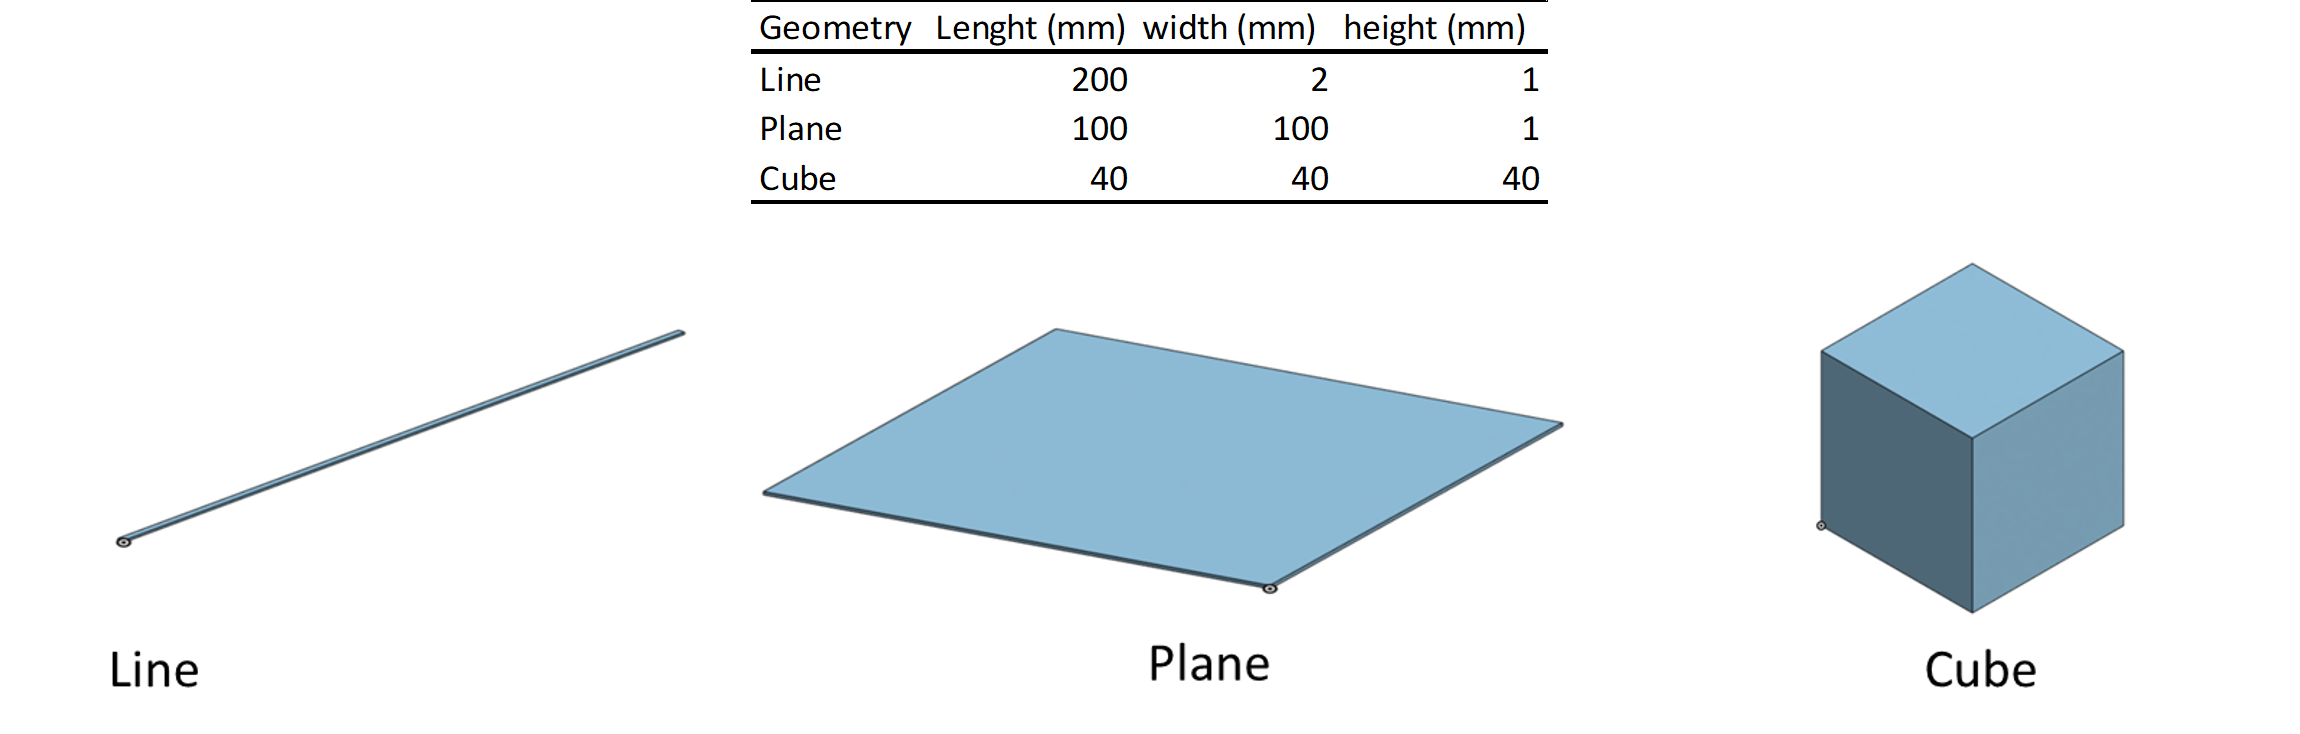
\includegraphics{figures/Figure-2.png}

}

\caption{\label{fig-cad}Dimensions and CAD models of the geometries used
for parameters optimization.}

\end{figure}

Four parameters were assessed: 1) nozzle temperature, 2) bed
temperature, 3) printing speed and 4) extrusion multiplier
\protect\hyperlink{ref-oberloier2022a}{{[}64{]}}. The initial parameters
for the line are presented in Table 1a while additional parameters were
obtained from preliminary experimental work shown in Table 1.b. Finally,
the PSO tuning parameters were found in the previous PSO work
\protect\hyperlink{ref-oberloier2022}{{[}63{]}} Table 1.c.

\begin{table}

\caption{\label{tbl-table1}table 1}\begin{minipage}[t]{\linewidth}
\subcaption{\label{tbl-table1-1}Line optimization initial parameters }

{\centering 

\tabularnewline

\centering\begingroup\fontsize{12}{14}\selectfont

\begin{tabular}{llrrll}
\toprule
Variable & Min & Max & Guess & True/False & Description\\
\midrule
\cellcolor{gray!6}{T1} & \cellcolor{gray!6}{255} & \cellcolor{gray!6}{270} & \cellcolor{gray!6}{260} & \cellcolor{gray!6}{TRUE} & \cellcolor{gray!6}{Temperature Zone 1 on GigabotX}\\
Tb & 80 & 90 & 85 & TRUE & Bed temperature\\
\cellcolor{gray!6}{Ps} & \cellcolor{gray!6}{10} & \cellcolor{gray!6}{25} & \cellcolor{gray!6}{15} & \cellcolor{gray!6}{TRUE} & \cellcolor{gray!6}{Printing Speed}\\
E & 0.5 & 2 & 1 & FALSE & Extrusion Multiplier\\
\bottomrule
\end{tabular}
\endgroup{}

}

\end{minipage}%
\newline
\begin{minipage}[t]{0.50\linewidth}
\subcaption{\label{tbl-table1-2}Fixed parameters to perform printing parameters optimization based on
PSO }

{\centering 

\tabularnewline

\centering\begingroup\fontsize{11}{13}\selectfont

\begin{tabular}{lll}
\toprule
Parameters & Value & Units\\
\midrule
\cellcolor{gray!6}{Layer height} & \cellcolor{gray!6}{0.5} & \cellcolor{gray!6}{mm}\\
Width & 2 & mm\\
\cellcolor{gray!6}{T2} & \cellcolor{gray!6}{230} & \cellcolor{gray!6}{°C}\\
T3 & 220 & °C\\
\cellcolor{gray!6}{Cooling} & \cellcolor{gray!6}{0} & \cellcolor{gray!6}{\%}\\
\addlinespace
Infill density & 2 & \%\\
\bottomrule
\end{tabular}
\endgroup{}

}

\end{minipage}%
%
\begin{minipage}[t]{0.05\linewidth}

{\centering 

~

}

\end{minipage}%
%
\begin{minipage}[t]{0.45\linewidth}
\subcaption{\label{tbl-table1-3}Recommended parameters for PSO tuning }

{\centering 

\tabularnewline

\centering\begingroup\fontsize{11}{13}\selectfont

\begin{tabular}{lr>{\raggedright\arraybackslash}p{4cm}}
\toprule
Variable & Value & Description\\
\midrule
\cellcolor{gray!6}{Kv} & \cellcolor{gray!6}{0.5} & \cellcolor{gray!6}{The emphasis given to the velocity component}\\
Kp & 1.0 & The emphasis given to a particle's personal best position\\
\cellcolor{gray!6}{Kg} & \cellcolor{gray!6}{2.0} & \cellcolor{gray!6}{The emphasis given to the swarm's group's best position}\\
\bottomrule
\end{tabular}
\endgroup{}

}

\end{minipage}%

\end{table}

\hypertarget{fused-granular-fabrication-fgf-}{%
\subsubsection{Fused Granular Fabrication
--FGF-}\label{fused-granular-fabrication-fgf-}}

To print the obtained raw material, a modified open-source printer with
three heat zones (Gigabot XL re:3D, Houston, TX, USA) was utilized as
illustrated in Figure~\ref{fig-gigabot}. The machine is a single screw
extrusion-based 3-D printer capable of direct printing pellets, flakes,
or granules, with a nozzle size of \(1.75~mm\). For this study, a chair
was printed to evaluate the material's ability to be 3-D printed and the
printer's capability to produce large objectslike furniture. The ideal
parameters determined for the cube geometry were employed to print the
final part.

\begin{figure}

{\centering 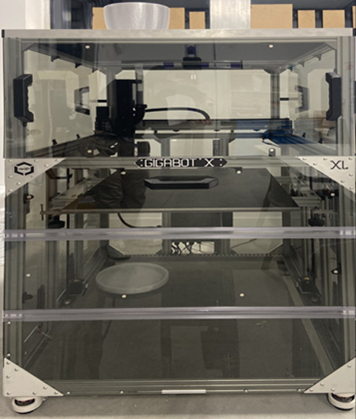
\includegraphics{figures/Figure_4_Giga.png}

}

\caption{\label{fig-gigabot}Fused granular fabrication printer Gigabot}

\end{figure}

\hypertarget{results-and-discussion}{%
\section{Results and discussion}\label{results-and-discussion}}

\hypertarget{material-characterization}{%
\subsection{Material characterization}\label{material-characterization}}

Both the polymeric components of the bottle and the blend were
characterized and analyzed to determine their properties using different
methods as described in the preceding section.

\hypertarget{material-particle-size-analysis-granulometry}{%
\subsubsection{Material particle size analysis
(granulometry)}\label{material-particle-size-analysis-granulometry}}

Previous studies demonstrated that particles with areas smaller than
\(22~mm^{2}\) were optimal for printing without experiencing jamming or
under-extrusion problems \protect\hyperlink{ref-woern2018}{{[}11{]}}.
However, our experiments revealed that particles with areas exceeding
\(10~mm^{2}\) caused clogging in the feeding system and auger screw of
the machine. As a result, granulometry analysis was performed using
three different mesh sizes.

\begin{figure}

\begin{minipage}[t]{0.57\linewidth}

{\centering 

\raisebox{-\height}{

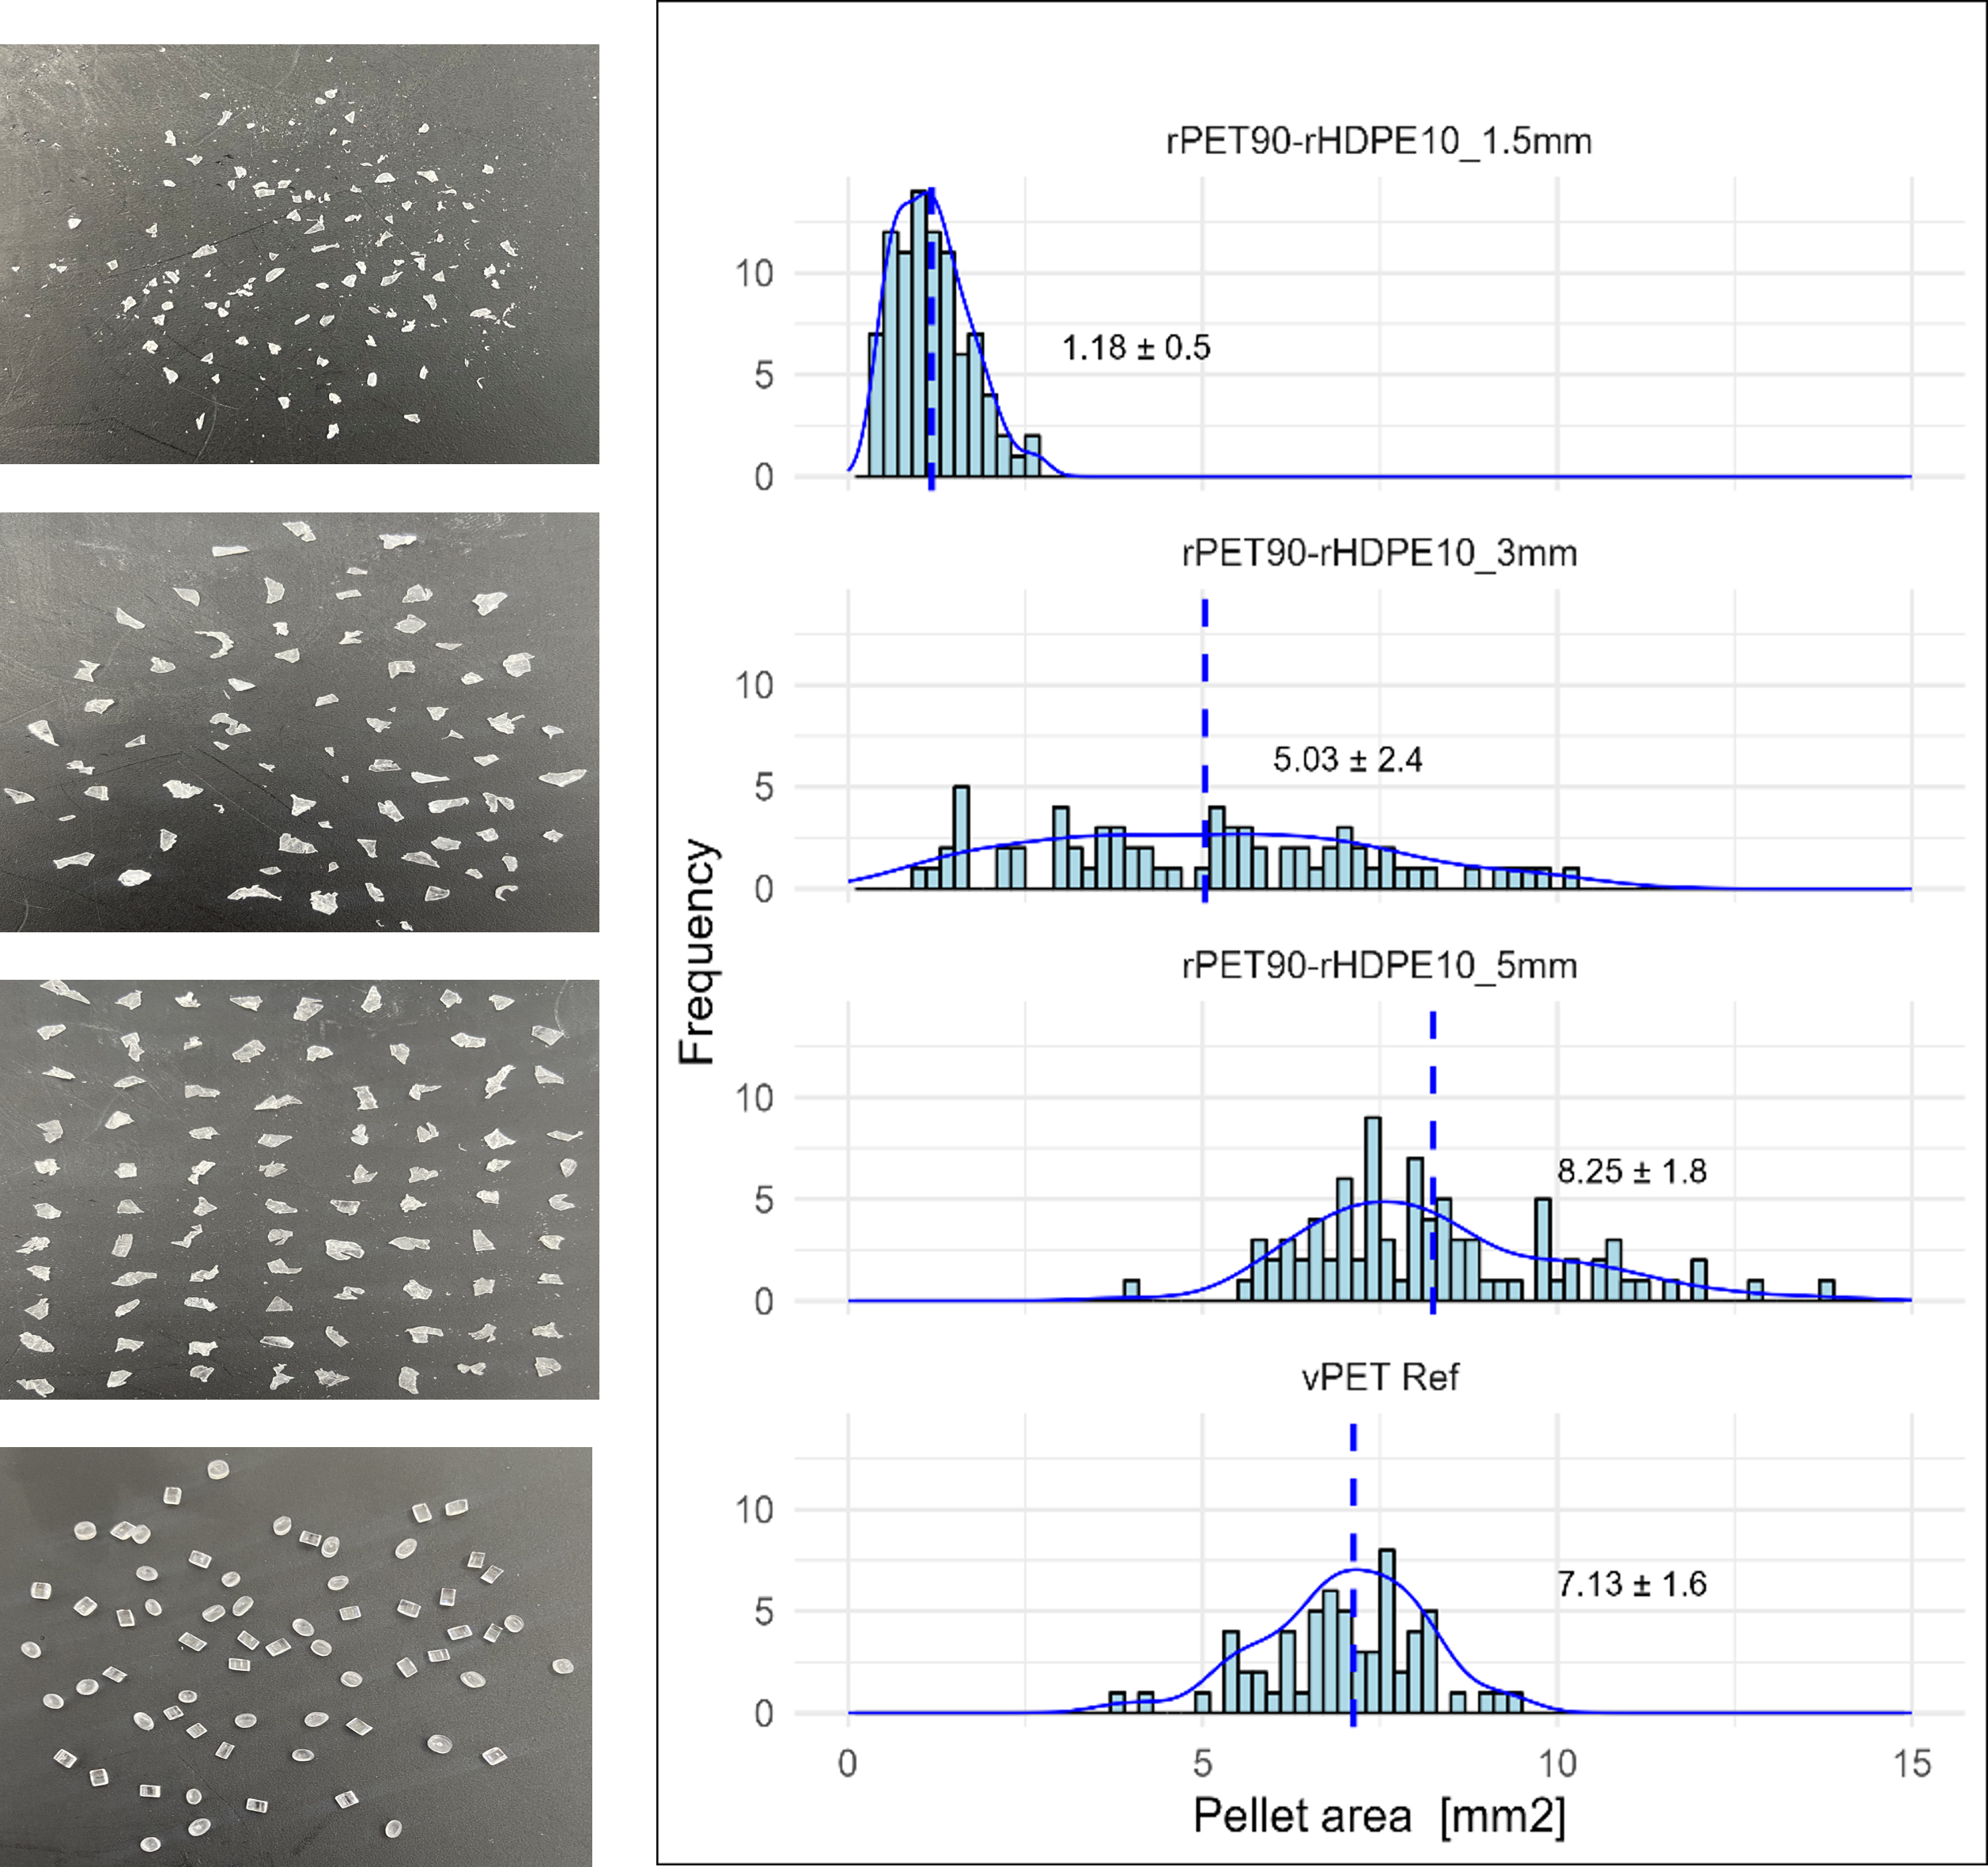
\includegraphics{figures/Figure_5_granulometry.png}

}

\caption{\label{fig-granulometry}Granulometry analysis}

}

\end{minipage}%
%
\begin{minipage}[t]{0.03\linewidth}

{\centering 

~

}

\end{minipage}%
%
\begin{minipage}[t]{0.40\linewidth}

{\centering 

\raisebox{-\height}{

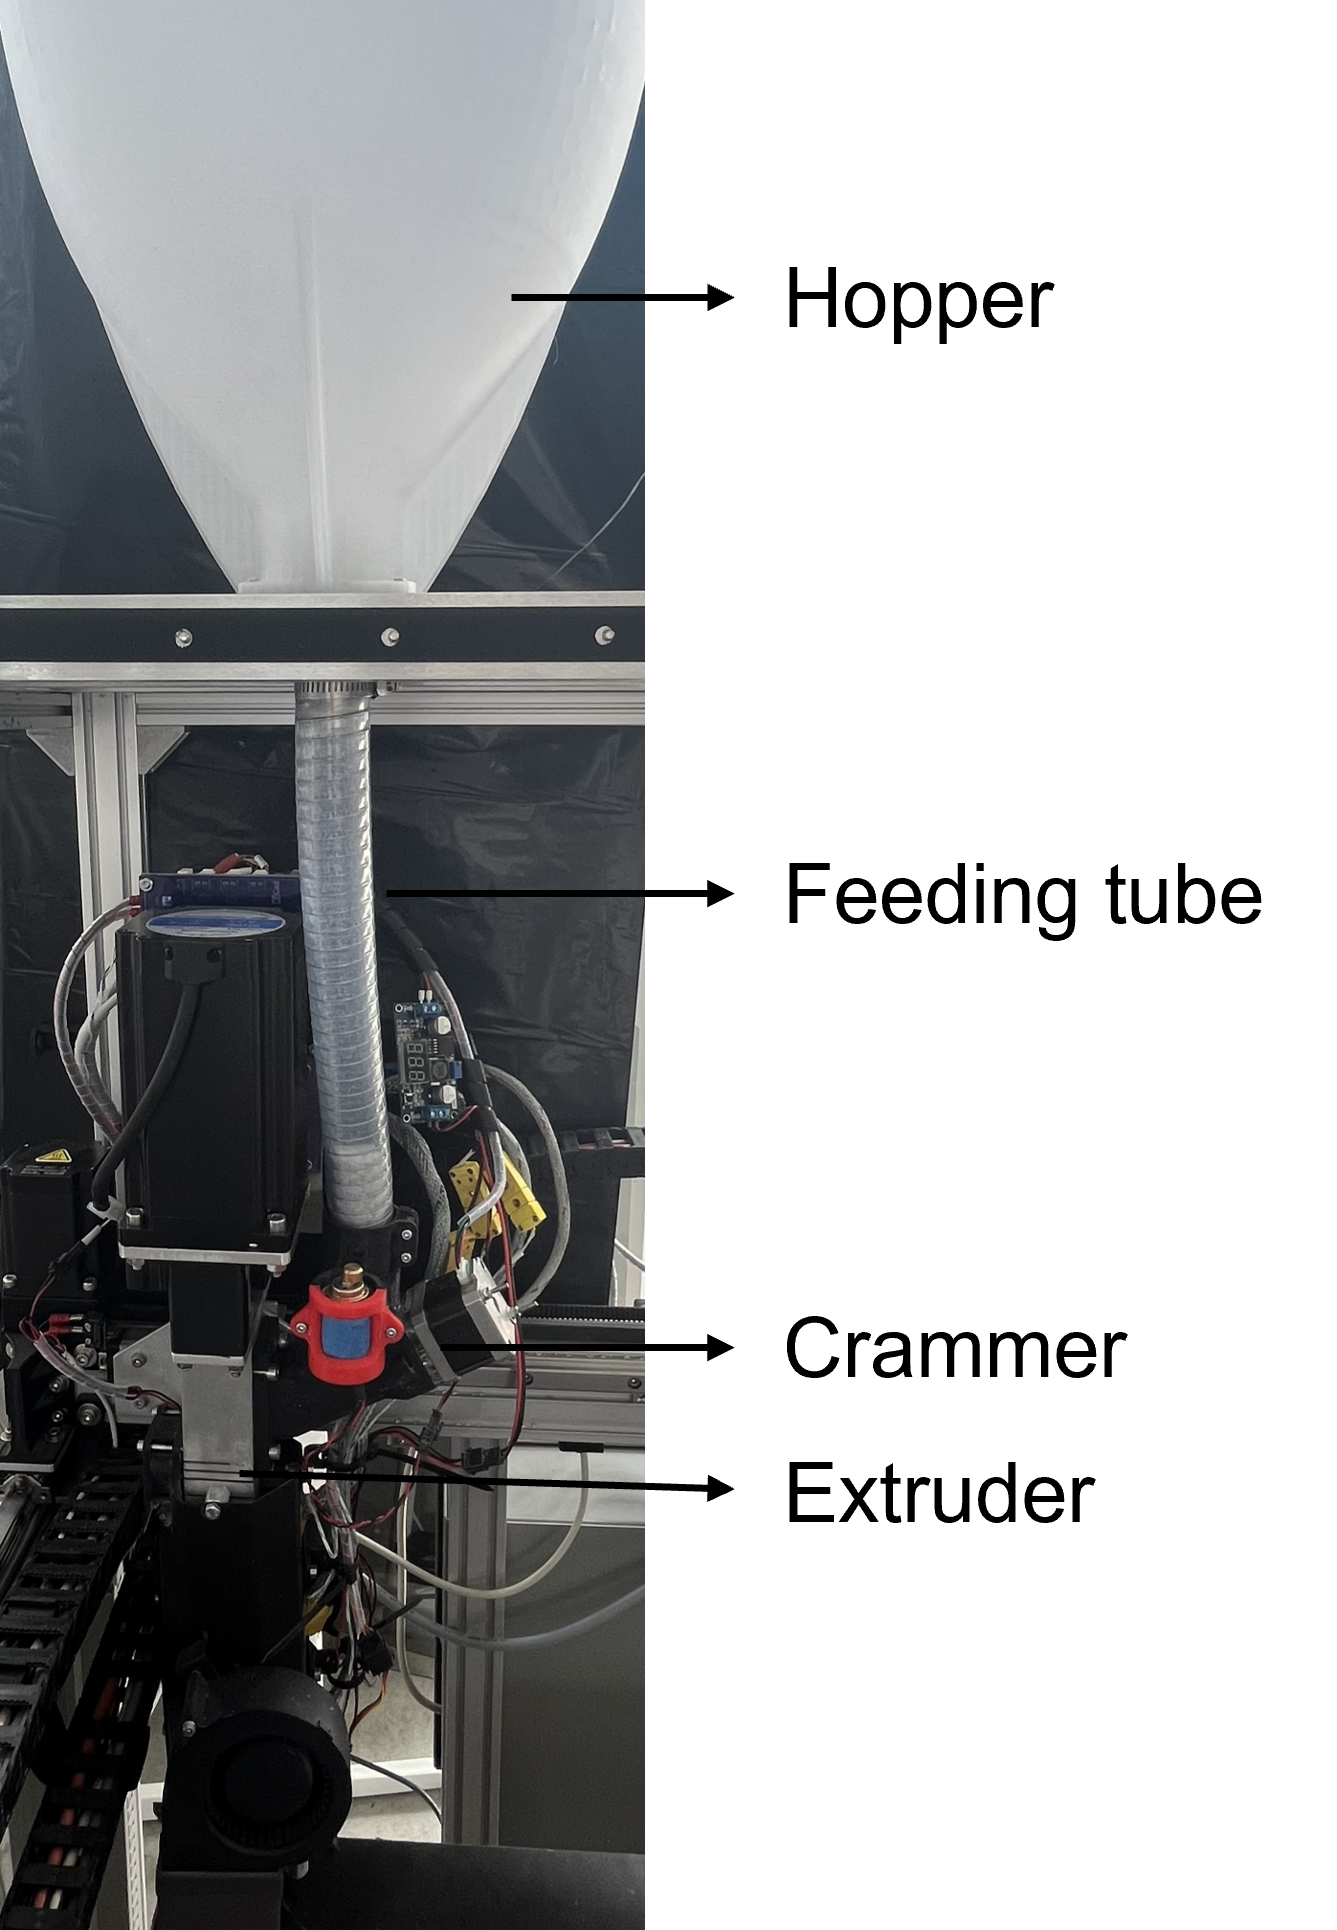
\includegraphics{figures/Figure_6_crammer.png}

}

\caption{\label{fig-crammer}Gigabot feeding system}

}

\end{minipage}%

\end{figure}

Figure~\ref{fig-granulometry} presents the obtained results, indicating
that particles sifted at \(5~mm\) exhibited an average area similar to
the reference. There are, however, particles with areas exceeding
\(9~mm^{2}\) caused blockages in the feeding and extrusion section.
Particles sifted to \(1.5~mm\) displayed a distribution ranging from 0
to approximately \(3~mm^{2}\), which was deemed too small for printing
purposes. The presence of these small particles can lead to their
complete melting in the initial heat zone, thereby impeding the smooth
flow of other particles and preventing the necessary pressure for
extruding the melted particles further down the screw. Although flakes
measuring 3 mm exhibited a more dispersed distribution and slightly
smaller area compared to the reference, they were found to be optimal
for printing.

The final objects, however, still showed under-extrusion issues. To
address this problem, a crammer was implemented
\protect\hyperlink{ref-little2020}{{[}55{]}} as presented in
Figure~\ref{fig-crammer}. The crammer physically pushes particles
towards the auger, facilitating their transfer from the feeding tube to
the extruder. After the crammer implementation the under-extrusion
issues were greatly reduced. It was concluded that flakes with areas
ranging from \(1.5~mm^{2}\) to \(10~mm^{2}\) were the most suitable for
printing when using a crammer to assist the feeding system.

\hypertarget{chemical-analysis-from-ftir}{%
\subsubsection{Chemical analysis from
FTIR}\label{chemical-analysis-from-ftir}}

Chemical structure information of the materials was obtained using FTIR
spectroscopy, which allowed the analysis of the characteristic spectral
bands of the polymers.

In the case of rPET (bottle) four distinct bands can be observed in
Figure~\ref{fig-FTIR}. The first band, located at \(1713 cm^{-1}\)
represent the \(C=O\) double bond. The second band, at \(1240 cm^{-1}\),
corresponds to the \(C-O\) single bond ester. The third band, at
\(1093 cm^{-1}\), is associated with band the methylene group and
vibrations of the ester bond. Lastly, a band at \(722 cm^{-1}\) which
represents the CH2 rocking bending vibration. Similar results were
reported in the literature for PET derived from recycled water bottles,
soda bottles, and food containers
\protect\hyperlink{ref-zander2018}{{[}29{]}}.

Regarding rHDPE (caps), four characteristic peaks were identified: the
C-H functional group bond at \(2915cm^{-1}\) and \(2847~cm^{-1}\), the
primary bending mode of the -CH2 at \(1465~cm^{-1}\) and the CH2 rocking
bending vibration at \(729 ~cm^{-1}\). The results obtained confirmed
the chemical structures of the starting materials. Additionally, no
other indicative resonances, apart from those associated with the
polymer structures were detected. This leads to the conclusion that
there were no significant amounts of additives or plasticizers present
in either of the samples. Moreover, the spectrum of the printed blend
(rPET90//rHDPE10) exhibited identical characteristic peaks to those
observed in the bottle, thus confirming the predominant presence of PET.
There are, however, noticeable differences between \(1000 ~cm^{-1}\) and
\(720 ~cm^{-1}\) as well as in the C-H bond (\(2915~cm^{-1}\) and
\(2847 ~cm^{-1}\) peaks), which confirm the presence of HDPE (cap). The
observed shift can be attributed to interactions between the two
materials.

\begin{figure}

{\centering 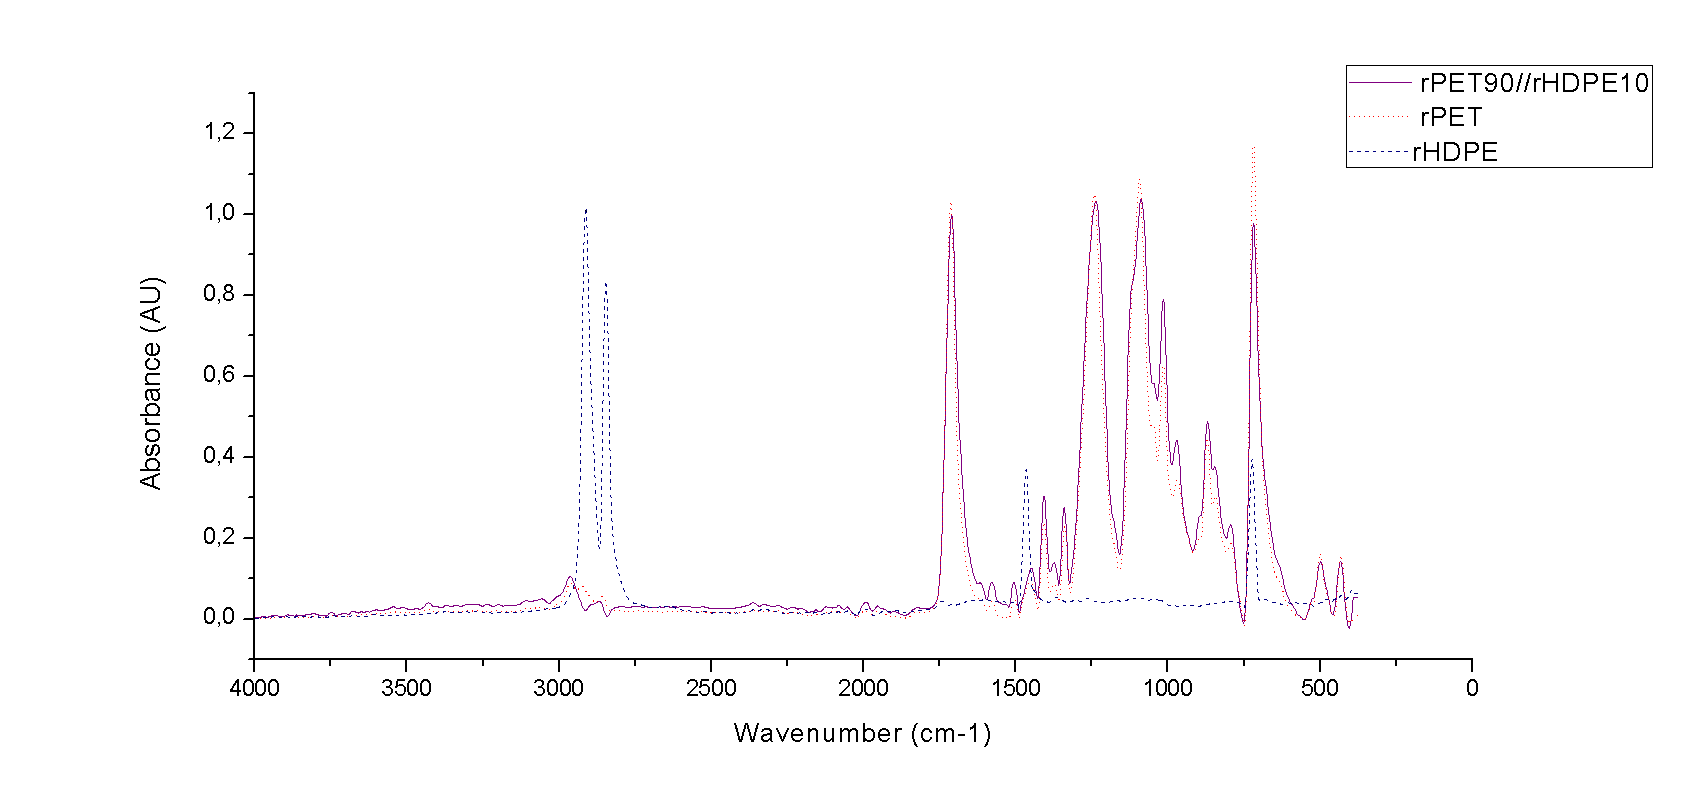
\includegraphics[width=0.9\textwidth,height=\textheight]{figures/Figure_7_FTIR.png}

}

\caption{\label{fig-FTIR}FTIR spectra of rPET, rHDPE, and their blend}

\end{figure}

\hypertarget{thermal-analysis-dsc}{%
\subsubsection{Thermal analysis DSC}\label{thermal-analysis-dsc}}

The thermal properties of both recycled materials and their blend were
characterized using DSC to establish a baseline for optimizing process
parameters of 3-D printing.

Two distinct endothermic peaks are observed in the representative
heating and cooling thermograms shown in Figure~\ref{fig-DCS}, for the
printed blend sample. These peaks are associated with the fusion of the
crystalline fractions of rHDPE and rPET, providing confirmation of the
immiscibility of both materials. Moreover, the enthalpy of fusion and
crystallization of the rHDPE in the blend is significantly reduced,
which can be attributed to the low percentage of HDPE present in the
blend. Furthermore, the presence of a cold crystallization peak in the
blend, but not in the individual polymers,suggests an interaction
between the two polymers. It is possible that the rHDPE acts as a
nucleating agent in this interaction. Table 2.lists the thermal
properties of rPET, rHDPE and rPET90//rHDPE10. The melting points of
rHDPE and rPET are 131.7 °C and 249.9 °C, respectively, which align with
previous findings in the literature
\protect\hyperlink{ref-vaucher2022}{{[}30{]}},
\protect\hyperlink{ref-lei2009}{{[}65{]}},
\protect\hyperlink{ref-chen2015}{{[}66{]}}. It is observed that the
melting and crystallization temperature of rPET increased, while that of
rHDPE slightly decreased. Furthermore, the crystallization of rPET was
found to be somewhat affected by the presence of rHDPE, resulting in a
3.5\% increase in degree of crystallization.This can be attributed to
the rHDPE acting as a germination point for crystallization
\protect\hyperlink{ref-vaucher2022}{{[}30{]}}. The slight changesin the
fusion-crystallization temperatures and degree of crystallinity of rPET
indicate an interaction of both polymers.

\begin{figure}

\begin{minipage}[t]{\linewidth}

{\centering 

\raisebox{-\height}{

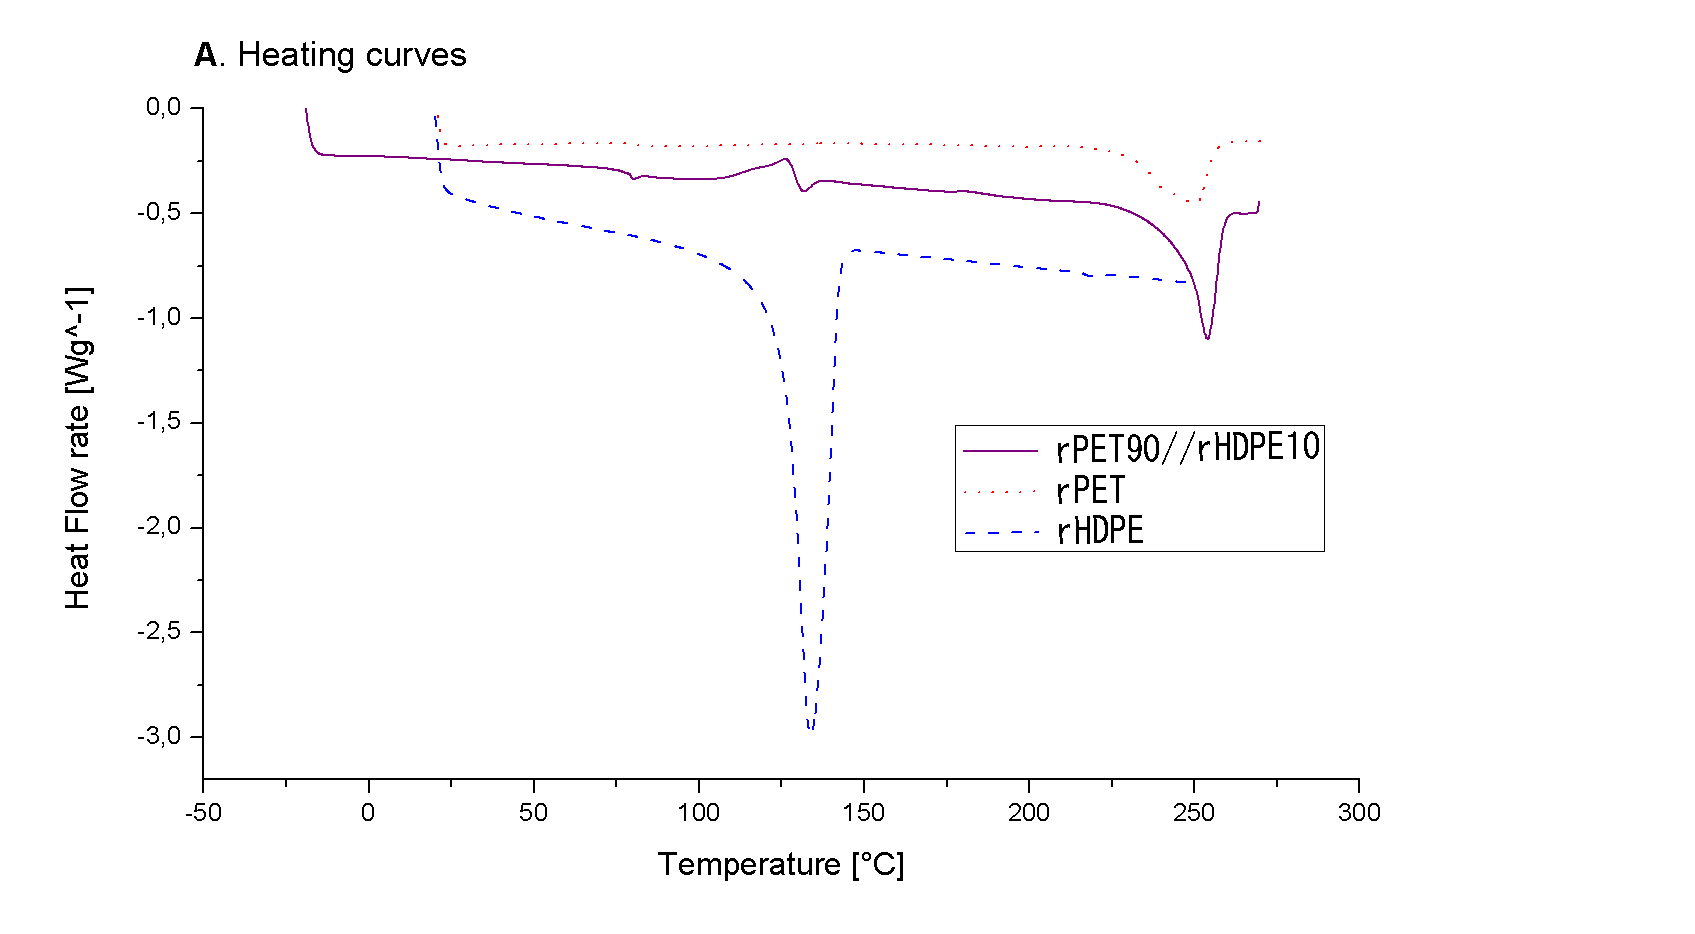
\includegraphics{figures/Figure_8a_DSC.png}

}

}

\subcaption{\label{fig-DCSa}Heating curves}
\end{minipage}%
\newline
\begin{minipage}[t]{\linewidth}

{\centering 

\raisebox{-\height}{

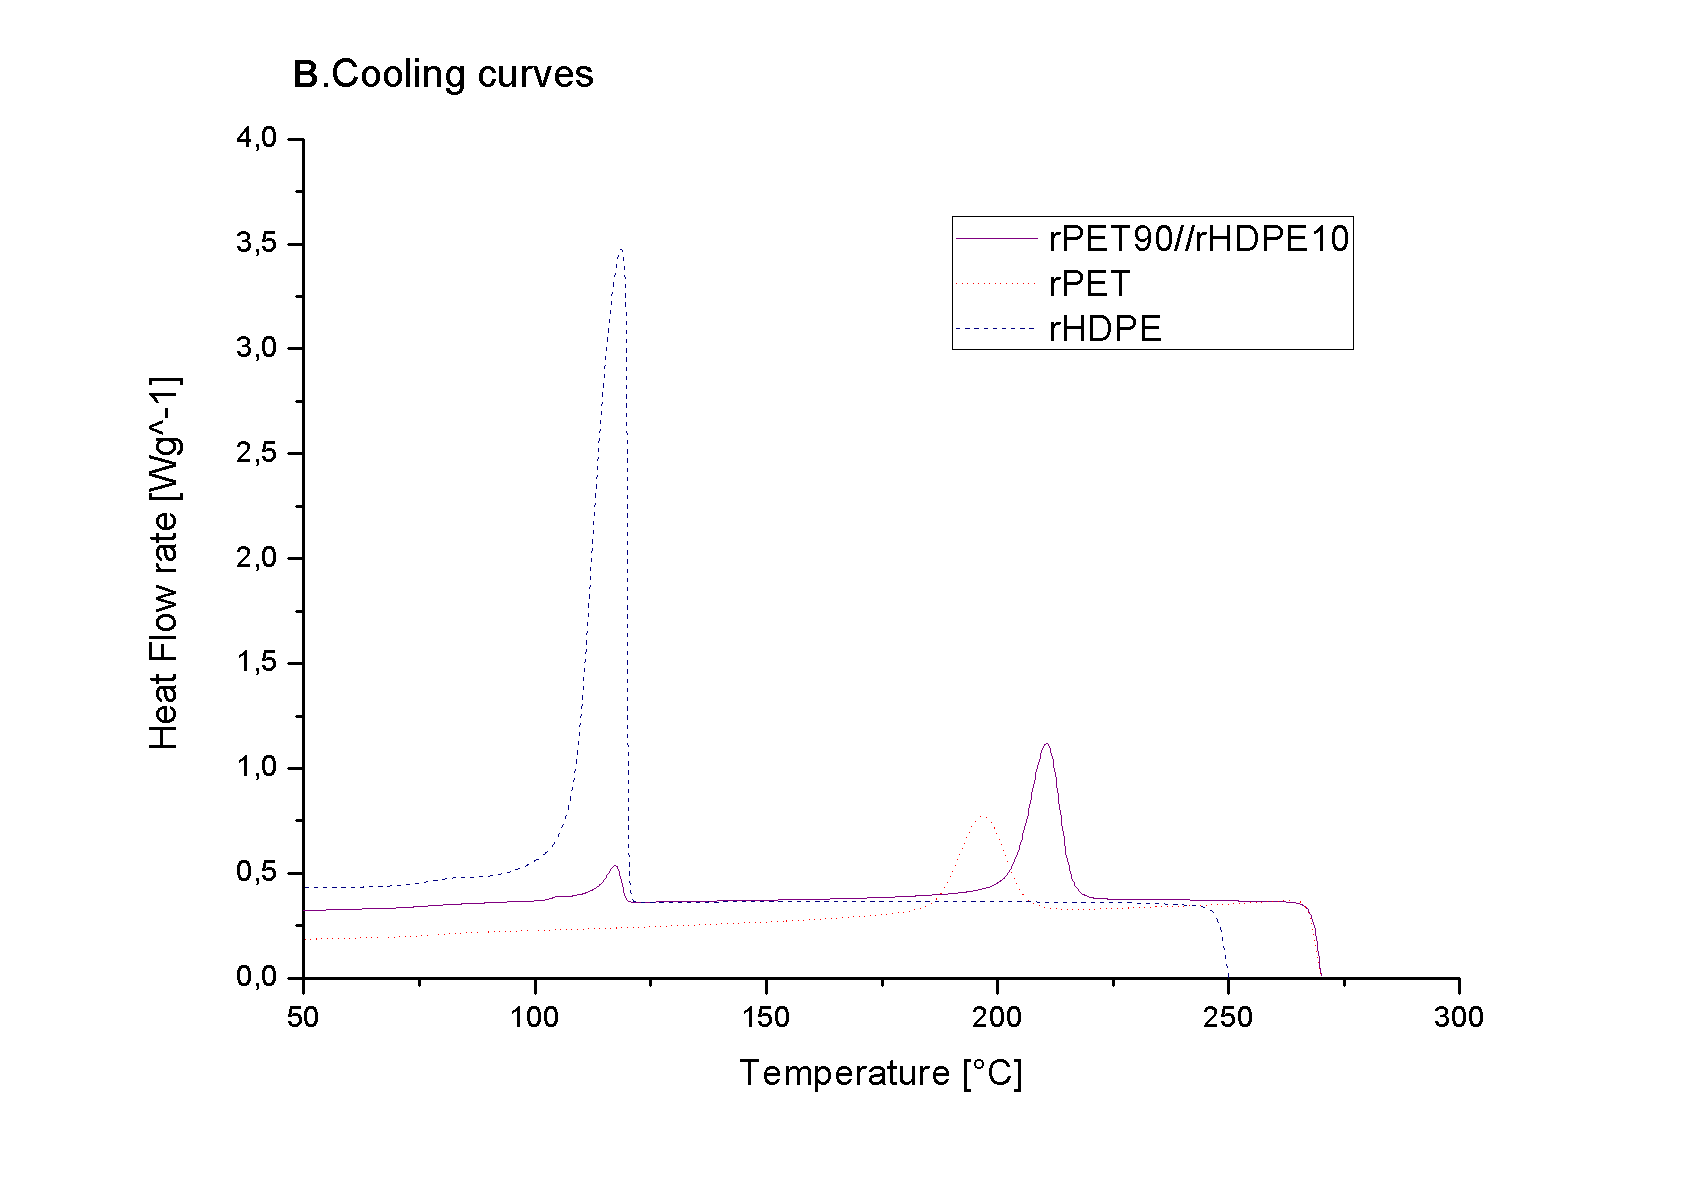
\includegraphics{figures/Figure_8b_DSC.png}

}

}

\subcaption{\label{fig-DCSb}Cooling curve}
\end{minipage}%

\caption{\label{fig-DCS}DSC thermograms of recycled materials and
blends}

\end{figure}

\begin{table}
\caption{Thermal analysis of rPET, rHDPE, and their blend}\tabularnewline

\centering\begingroup\fontsize{8}{10}\selectfont

\begin{tabular}[t]{llllllll}
\toprule
\multicolumn{1}{c}{ } & \multicolumn{1}{c}{Glass transition} & \multicolumn{2}{c}{Melting} & \multicolumn{3}{c}{Crystallization } & \multicolumn{1}{c}{\% Crystallinity} \\
\cmidrule(l{3pt}r{3pt}){2-2} \cmidrule(l{3pt}r{3pt}){3-4} \cmidrule(l{3pt}r{3pt}){5-7} \cmidrule(l{3pt}r{3pt}){8-8}
Sample & Tg (°C) & Tm  (°C ) & ΔHm (J/g) & Tc  (°C ) & ΔHc (J/g) & ΔHcc (J/g) & Xc\\
\midrule
\cellcolor{gray!6}{rPET} & \cellcolor{gray!6}{82} & \cellcolor{gray!6}{249.9} & \cellcolor{gray!6}{32.3} & \cellcolor{gray!6}{196.7} & \cellcolor{gray!6}{33.3} & \cellcolor{gray!6}{-} & \cellcolor{gray!6}{23.1}\\
rHDPE & - & 133.8 & 172 & 118.7 & 158.2 & - & 58.7\\
\cellcolor{gray!6}{rPET90/rHDPE10} & \cellcolor{gray!6}{77 / -} & \cellcolor{gray!6}{254/131.7} & \cellcolor{gray!6}{40.3/1.30} & \cellcolor{gray!6}{210.6/117.4} & \cellcolor{gray!6}{37.9/6.7} & \cellcolor{gray!6}{6.8} & \cellcolor{gray!6}{26.6 / 18.8}\\
\bottomrule
\end{tabular}
\endgroup{}
\end{table}

\hypertarget{rheology-mfi}{%
\subsubsection{Rheology MFI}\label{rheology-mfi}}

The melt flow index of the flakes was determined, enabling a fast and
practical screening of the viscosity of the material. Based on the DSC
results, the initial temperature for the MFI test was 250°C. However,
the material did not flow reliably at this temperature, so it was
increased by 5°C to enable the determinationof the melt flow index of
the rPET90//rHDPE10 blend. A temperature of 260°C was also tested,
however, the material flowed too rapidly, making difficult to obtain
reliable measurements. The MFI tests were performed three times and the
results for the rPET90//rHDPE10 blend showed medium MFI of 39.4± 2.4
g/10min. This value is consistent with similar values reported in the
literature for rPET
\protect\hyperlink{ref-bustosseibert2022}{{[}67{]}}--\protect\hyperlink{ref-Langer2020}{{[}69{]}}.
This result suggest that addition of low percentage of HDPE does not
significantly impact the MFI value of rPET. Since the material flowed at
a temperature of 255°C in the MFI test, this temperature was used as the
input temperature for optimizing the parameters of the 3-D printer.

\hypertarget{density-1}{%
\subsubsection{Density}\label{density-1}}

The density provides valuable information for estimating the cost,
material usage, time consumption, and weight of the printed object in
the slicer. This information is useful to determine the accurate
printing parameters using the PSO experimenter, as the fitness of the
object is calculated based on its dimensional accuracy and weight.
Hence, density plays a significant role in determining the weight of the
geometries.

After conducting calculations and measuring the rPET90//rHDPE10 injected
object, it was determined that the density of the material is 1.13
\(g/cm^{3}\). The inclusion of HDPE in the matrix polymer resulted in a
slight decrease in density, which is a common occurrence when a polymer
is mixed with a lower-density polymer. However, if we consider a
PET/HDPE blend with a mass ratio of 90/10, the calculated theoretical
density would be 1.32 \(g/cm^{3}\). The observed decrease of 14\% in the
results could be attributed to factors, such as experimental conditions
and manual measurements.

\hypertarget{particle-swarm-optimization-pso-experimenter}{%
\subsection{Particle swarm optimization (PSO)
Experimenter}\label{particle-swarm-optimization-pso-experimenter}}

Geometries were 3-D printed by adjusting the parameters using the PSO
Experimenter software. The fitness function is defined by the weighted
sum of the dimensional measurements (length, width, height, and weight)
of the printed object. A fitness value below 0.1 was consider desirable.
In the software five particles were established for each iteration,
resulting in five different parameter combinations being printed in each
iteration.

After six iterations and a total of thirty lines printed, the first
geometry (line) achieved a fitness value of less than 0.1. The optimal
parameters for this geometry are listed in column two of
Table~\ref{tbl-table3} and images of the resulting geometries are
illustrated in Figure~\ref{fig-geometries} .

\begin{figure}

{\centering 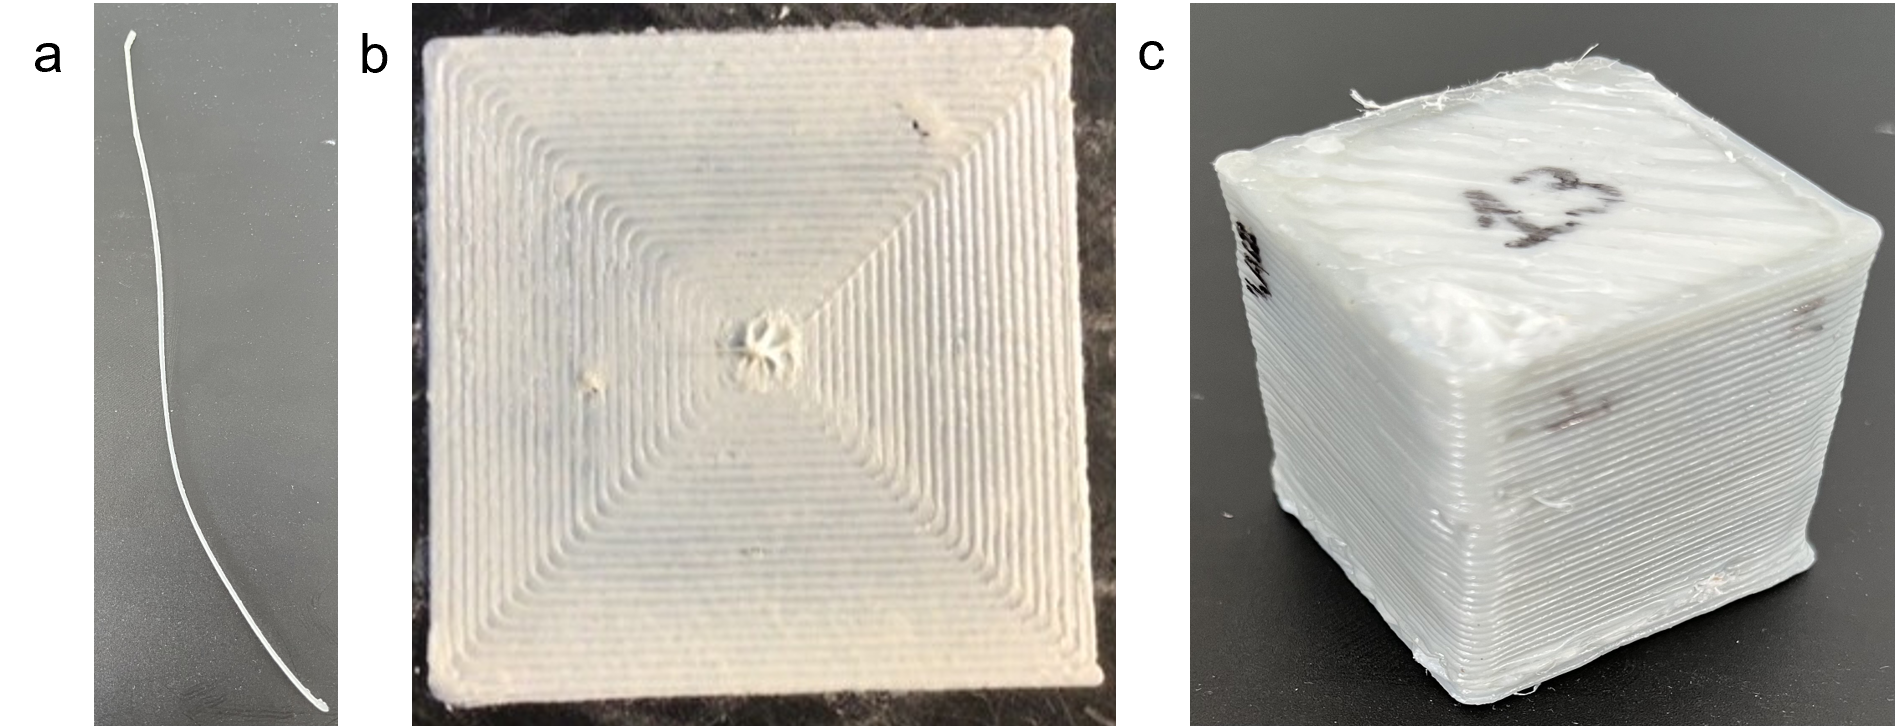
\includegraphics{figures/Figure_9_geometries.png}

}

\caption{\label{fig-geometries}Images of the resulting geometries a)
line, b) plane, c) cube}

\end{figure}

Afterwards, these parameters were used as initial guesses for plane
geometry, which achieved the desired fitness in the first iteration.
Similarly, cubes were printed using the plane ideal parameter as the
initial guess, and optimal parameters, were found in the first
iteration. The results showed a significant decrease in printing speed,
as the geometry complexity increased. Moreover, the cube geometry
required a higher extrusion multiplier to fill gaps and overcome
under-extrusion problems. The optimization of parameters for the three
geometries took approximately 10h reducing the experimental time,
compared to conventional methods. According to
\protect\hyperlink{ref-oberloier2022}{{[}63{]}}, this experimentation
time can be reduced by 97\%. Indeed, the effectiveness of PSO in finding
global optimum parameters is high, especially in cases with a large or
complex design space \protect\hyperlink{ref-saad2019a}{{[}70{]}},
\protect\hyperlink{ref-selvam2020}{{[}71{]}}.

Additionally, PSO converge to optimum solutions with fewer iterations
than DoE methods \protect\hyperlink{ref-zhang2015}{{[}72{]}}. Combining
PSO with other meta-heuristic methods has demostrated higher ability to
predict and optimize parameters (e.g.~minimize surface
roughness\protect\hyperlink{ref-shirmohammadi2021}{{[}73{]}},
compressive strength and porosity of scaffolds
\protect\hyperlink{ref-asadi-eydivand2016}{{[}74{]}},and mechanical
properties\protect\hyperlink{ref-raju2019}{{[}75{]}}). However, DoE
methods are still widely used as they provide insight into the effects
of individual design parameters and their interactions while the ability
to find interaction between the variables is not possible using PSO. In
the beginning of optimization experiments, the understanding the process
technique and function settings might be complex. The methodology used
in this study, however, was easy to implement and the software used was
free, open source, and user-friendly, which reduced the initial
difficulty. Therefore, PSO was demonstrated to be an effective and
highly accurate prediction technique for finding the initial optimum
parameters for rPET90//rHDPE10 material for FGF/FPF.

Based on the result, it is evident that the optimal parameters for
printing may vary depending on the object and each parameter has its own
variation. One possible hypothesis is that the geometry of the object
could influence the assignment of parameters and this effect might be
more noticeable in large printings, yet further investigation is
required to confirm this hypothesis. There are several physical
mechanisms at play that are expected to alter the optimal printing
parameters based on size and geometry of the object. For example, the
cooling time and temperature history of a voxel will depend on the
geometry of the printed object
\protect\hyperlink{ref-cleeman2022}{{[}76{]}}. Thus, to maintain a
consisten thermal history the printing parameters must be ajusted as the
geometry changes. This thermal history can also have more subtle
effects, such asimpacting the degree of crystallization even in the case
of PLA \protect\hyperlink{ref-wijnen2018}{{[}77{]}}.

In addition, the effects of material extrusion are magnified with scale,
including the impact of thermal expansion and contraction. Small changes
in contraction during cooling may cause acceptable distortions for small
prints, but these are magnified for larger prints (e.g.~causing
deformation and in the worst cases delamination or loss of bed
adhesion)\protect\hyperlink{ref-shah2019}{{[}78{]}}. Although,
\protect\hyperlink{ref-roschli2019}{{[}79{]}} showed the obstacles and
possible solutions of the large-scale AM according to the way the parts
are designed the incidence of the geometry in the printing parameters
needs far more detailed future studies. Specifically better models for
mapping 3-D printing parameter optimization of small printed objects to
large-volume objects are needed.

\hypertarget{tbl-table3}{}
\begin{table}
\caption{\label{tbl-table3}Ideal printing parameters for fused granule fabrication of waste PET and
HDPE blend made from shredded whole plastic water bottles }\tabularnewline

\centering\begingroup\fontsize{10}{12}\selectfont

\begin{tabular}[t]{llllll}
\toprule
Variable & Line value & Planes value & Cube value & Δ & Units\\
\midrule
\cellcolor{gray!6}{T1} & \cellcolor{gray!6}{258} & \cellcolor{gray!6}{263} & \cellcolor{gray!6}{264} & \cellcolor{gray!6}{6 ±3.2} & \cellcolor{gray!6}{°C}\\
Tb & 86 & 82 & 84 & 4±2 & °C\\
\cellcolor{gray!6}{Ps} & \cellcolor{gray!6}{21} & \cellcolor{gray!6}{14} & \cellcolor{gray!6}{10} & \cellcolor{gray!6}{11±5.6} & \cellcolor{gray!6}{mm/s}\\
E & 1.07 & 0.87 & 1.32 & 0.5±0.3 & -\\
\bottomrule
\end{tabular}
\endgroup{}
\end{table}

\hypertarget{functional-object-print}{%
\subsection{Functional object print}\label{functional-object-print}}

The final parameters for print the case study product were determined
based on the ideal paraeters found for the cube geometry.However, the
print speed was ajusted to decrease the printing time and prevent
delamination. This adjustment was made in accordance with the PSO
results, which indicated that the material can be printed at a speed
range of 10 to 20 \(mm/s\). Increasing the printing speed reduces the
cooling time between the layers,thereby minimizing the risk of
delamination \protect\hyperlink{ref-roschli2019}{{[}79{]}}, This is
particularly important for larger objects, as delamination tends to be
more pronounced in such cases.

The Gigabot X successfully produced a piece of furniture from
multi-material recycled water bottles that included mixing HDPE and PET
as shown in Figure~\ref{fig-child} a.

The printing quality is acceptable as a prototype, proving the machine's
capacity to print large-scale functional objects. The chair was able to
comfortably hold a child with a mass of 20 kg, as shown in
Figure~\ref{fig-child} f.~However, further evaluation is needed for the
material used in the printing process. the printed object showed weak
bond strength between the adjacent layers resulting in delamination, as
seen in Figure~\ref{fig-child} b . This could be attributed to the
difference in chemical properties of the materials, their immiscibility
\protect\hyperlink{ref-chu2022}{{[}80{]}},
\protect\hyperlink{ref-william2021}{{[}81{]}}, high crystallinity
\protect\hyperlink{ref-verma2023}{{[}82{]}} and the large volume of the
object as delamination issues were more prominent during the printing of
the chair compared to the parameters optimization process. The
delamination observed in larger objects can be attributed to the rapid
cooling of the layers before the material is once again deposited. This
is in contrast to cube printing, where the smaller surface area allows
better layer adhesion before complete cooling. Even popular 3-D printing
materials like PLA can be affected by this issue, as observed from the
print surface \protect\hyperlink{ref-wijnen2018}{{[}77{]}}. To address
the delamination problem and improve material properties, the addition
of agents that reduce could be benificial
\protect\hyperlink{ref-kramer1994}{{[}83{]}}--\protect\hyperlink{ref-inoya2012}{{[}85{]}}.
This can enhance interfacial bonds through polymer modification
\protect\hyperlink{ref-gao2021}{{[}86{]}} and viscosity reduction
\protect\hyperlink{ref-ko2019}{{[}87{]}}. Additionally,we observed
printing warping problems (Figure~\ref{fig-child} c), which are likely
caused by the high crystallization rates of HDPE. we tested the use of
Magigoo adhesive (Thougth3D Ltd., Paola, Malta) and the addition of a
brim to improve bed adhesion, yet these solutions did not completely
resolve the problem. A previous study showed that the use of a building
plate made of thermoplastic elastomer SEBS allowed the adhesion of the
plastic and facilitated easy detachment of the printed object without
any breakage or damage
{[}\protect\hyperlink{ref-schirmeister2019.This}{\textbf{schirmeister2019.This?}}
suggests a potencial solution that should be further evaluated in future
work. Another visible issue present in the close angles of the printed
object was the shrinkage (Figure~\ref{fig-child} d) which occurs during
solidification and particularly upon polymer crystallization. Moreover,
it is well-known that PET has hygroscopic tendencies and easily absorbs
moisture from the temperature, which makes it difficult to extrude
\protect\hyperlink{ref-bustosseibert2022}{{[}67{]}}. As result, it is
likely to break down in the presence of water, lowering the quality of
the print. Prior to printing the chair some samples exhibited brittle
behavior and void formation therefore, the material was consistently
dried and the hopper was kept closed to prevent moisture from entering
the environment.These measures helped to ensure a more suitable material
for printing.Additionally, there are visible vibration and ringing
problems (Figure~\ref{fig-child} e) caused by the machine upgrades.Both
acceleration and jerk (the maximum value of instantaneous speed change)
require finer tuning to resolve these issues.

\begin{figure}

{\centering 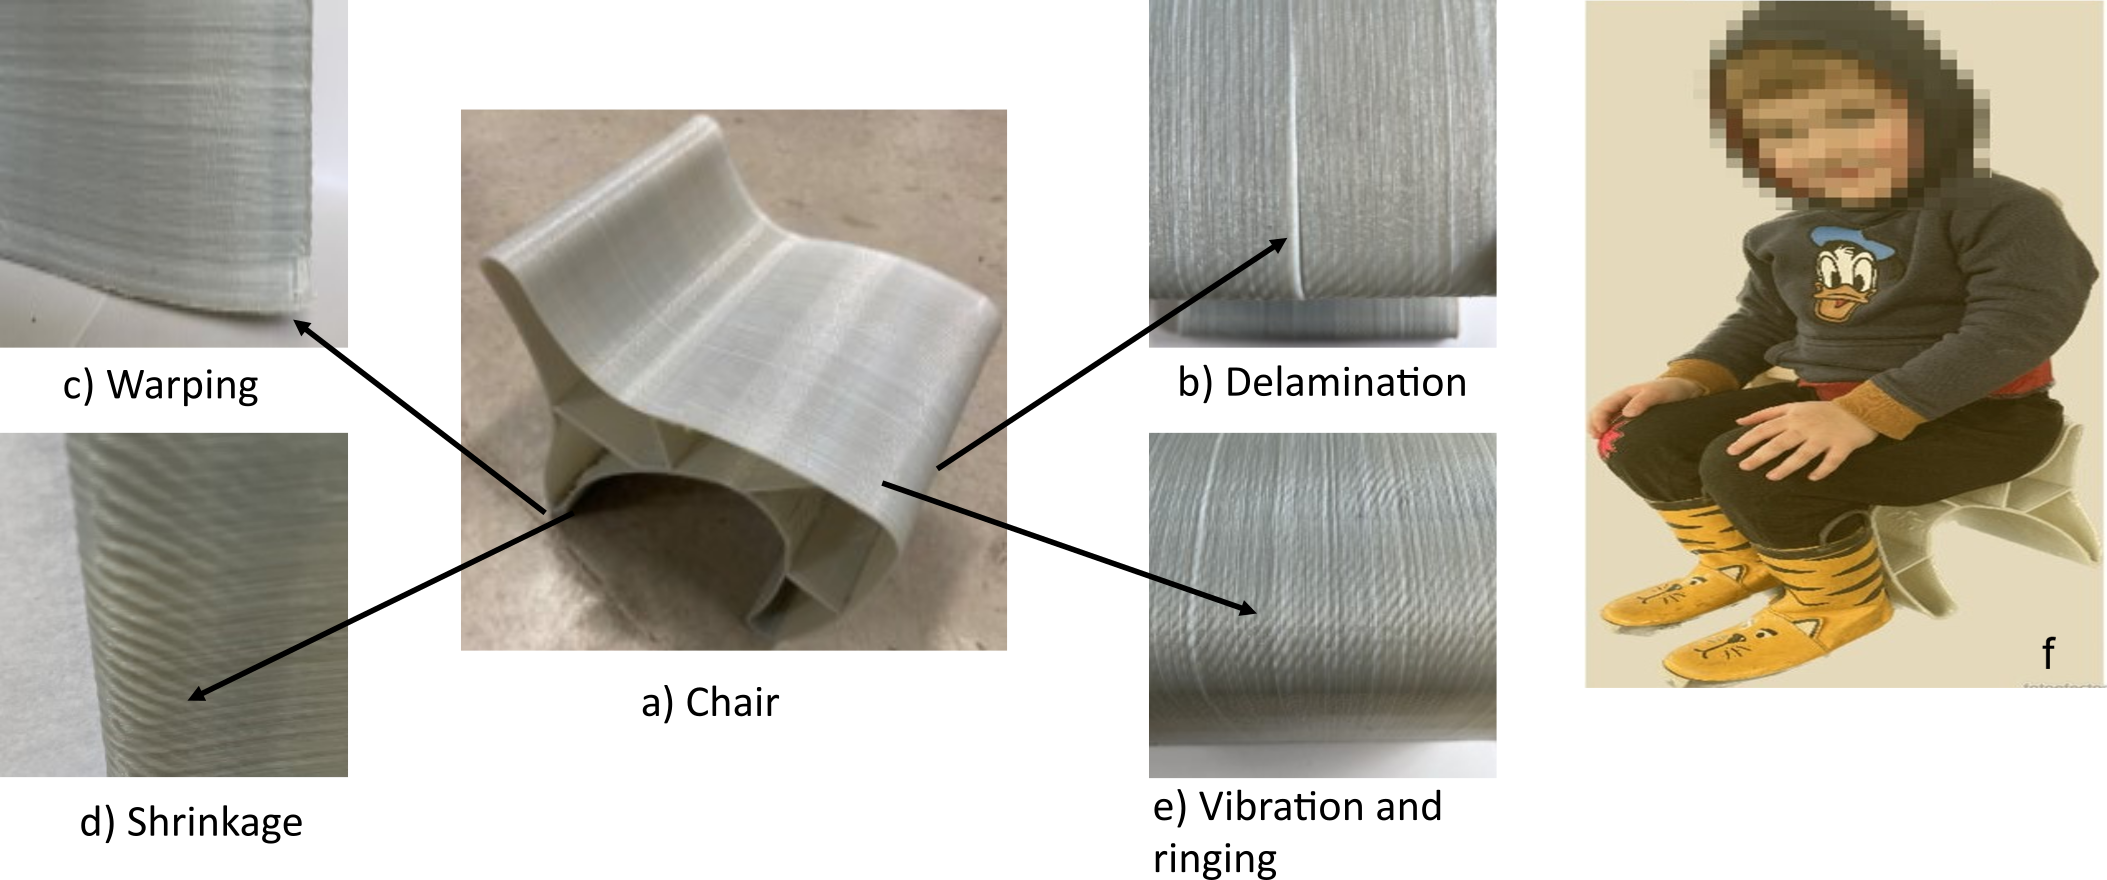
\includegraphics{figures/Figure6.png}

}

\caption{\label{fig-child}Finished children's chair and printing issues}

\end{figure}

\hypertarget{cost-and-environmental-impact}{%
\subsubsection{Cost and environmental
impact}\label{cost-and-environmental-impact}}

The printing process took 10 hours and the printed object weighs 840
grams. Due to the found optimized speed being low, the printing rate (
grams per hour) is low considering the machine that pellet printers have
a typical throughput of 220 g to 9 kg per hour. To improve the printing
time, upgrading the the extruder motor to a more powerful would be
benefitial. Besides, the energy required for 10 hours of 3-D printing
was found to be 6 kW-hr resulting in a production cost of
\textasciitilde1.2 € in function of the electricity cost in France, and
does not include the material cost, as the bottles used were obtained
from post-consumer waste. When labor costs are not included, the price
was significant reduced (\textasciitilde88\%) compared to the low-cost
options available in the market.

The economics of fabricating the case study product remained competitive
even when using recycled plastic pellets or shreds, which are avalable
on the market for prices ranging from 1-10 €/kg. However, it is
important to note that labor, maintenance, and machine devaluation were
not considered in the final price. These factors should be considered in
future work to ensure a comprehensive economic evaluation.

Regarding the environmental impact, this study does not evaluate the
entire life cycle of the printed object. However, various scientific
studies have already shown the feasibility of distributed recycling
\protect\hyperlink{ref-santander2020}{{[}17{]}},
\protect\hyperlink{ref-kerdlap2022}{{[}88{]}}. A comparison between
conventional and distributed manufacturing in terms of energy
consumption and emissions has been conducted
\protect\hyperlink{ref-Kreiger2013}{{[}89{]}}. Other studies have
examined the environmental performance of AM
\protect\hyperlink{ref-garcia2018}{{[}90{]}},
\protect\hyperlink{ref-colorado2020a}{{[}91{]}} and the appearance of
DRAM as a source of raw material for diverse 3-D printers coming from
post-consumer plastic waste in the form of either filament
\protect\hyperlink{ref-mohammed2017a}{{[}27{]}},
\protect\hyperlink{ref-hart2018}{{[}92{]}}--\protect\hyperlink{ref-mikula2021}{{[}94{]}}
or granules \protect\hyperlink{ref-alexandre2020}{{[}52{]}}.

Additionally, \protect\hyperlink{ref-caceres-mendoza2023}{{[}95{]}} have
developed a comprehensive life cycle assessment of a DRAM system
focusing on the production of PLA filament, comparing virgin and
recycled materials. The findings of their environmental analysis
revealed a analysis revealed a reduction of approximately 97\% in the
production impacts, including climate change, fossil depletion, water
depletion, and potential eutrophication, when using recycled filament as
opposed to virgin filament. It is important to note that these results
are subject to the energy supply and might vary depending on the
geographical location.

\hypertarget{conclusion-and-future-work}{%
\section{Conclusion and future work}\label{conclusion-and-future-work}}

This study examined the feasibility of using mixed post-consumer waste
as a feedstock material for direct 3-D printing without the need of
compatibilization. The results demostrated the potential of mixing solid
waste plastics (PET/HDPE) to be used as feedstock material, as evidenced
by successfully printing a water bottle using two incompatible polymers
from the cap and body of the bottle. Additionally, the results found
that a large-scale FGF 3-D printer was capable of producing
cost-effective functional object using these mixed waste PET/HDPE
plastics. However, further research is necessary to analyze the
mechanical properties of the material and explore the use of
compatibilizers that can enhance the interphase tension between plastics
and reduce their crystallinity. These measures could potentially improve
and enhance the properties of both the material and the 3-D printed
parts.

These considerations become increasingly important as the size of the
3-D printed part increases. The improvement of the material science of
this approach can also offer an opportunity to improve the quality of
the printing time, reduce energy consumption of the machine, and improve
the economic viability of DRAM using mixed plastic waste.

In addition, future work could assess the different combinations or
blends of commodity plastics with or without the use of compatibilizers,
to determine their printability. This investigation could lead ti the
elimination of the selection/sorting process. In the same way, the
development of a methodology that ensure process reproducibility, even
in areas with limited infrastructure opens up the potential for plastic
revalorization using DRAM.

\hypertarget{declaration-of-competing}{%
\section*{Declaration of competing}\label{declaration-of-competing}}
\addcontentsline{toc}{section}{Declaration of competing}

The authors declare that they have no known competing financial
interests or personal relationships that could have appeared to
influence the work reported in this paper.

\hypertarget{acknowledgments}{%
\section*{Acknowledgments}\label{acknowledgments}}
\addcontentsline{toc}{section}{Acknowledgments}

This project has received funding from the European Union's Horizon 2020
research and innovation program under grant agreement No 869952. The
authors thank the LUE program for the financing of the thesis, the
Lorraine Fab Living lab platform and the Thompson endowment.

\newpage

\hypertarget{references}{%
\section*{References}\label{references}}
\addcontentsline{toc}{section}{References}

\setstretch{1.1}

\hypertarget{refs}{}
\begin{CSLReferences}{0}{0}
\leavevmode\vadjust pre{\hypertarget{ref-evode2021}{}}%
\CSLLeftMargin{{[}1{]} }%
\CSLRightInline{N. Evode, S. A. Qamar, M. Bilal, D. Barceló, and H. M.
N. Iqbal, {``Plastic waste and its management strategies for
environmental sustainability,''} \emph{Case Studies in Chemical and
Environmental Engineering}, vol. 4, p. 100142, Dec. 2021, doi:
\href{https://doi.org/10.1016/j.cscee.2021.100142}{10.1016/j.cscee.2021.100142}.}

\leavevmode\vadjust pre{\hypertarget{ref-macarthur2017}{}}%
\CSLLeftMargin{{[}2{]} }%
\CSLRightInline{E. MacArthur, {``Beyond plastic waste,''}
\emph{Science}, vol. 358, no. 6365, pp. 843--843, Nov. 2017, doi:
\href{https://doi.org/10.1126/science.aao6749}{10.1126/science.aao6749}.}

\leavevmode\vadjust pre{\hypertarget{ref-geyer2020}{}}%
\CSLLeftMargin{{[}3{]} }%
\CSLRightInline{R. Geyer, {``Chapter 2 - {Production}, use, and fate of
synthetic polymers,''} in \emph{Plastic {Waste} and {Recycling}}, T. M.
Letcher, Ed., {Academic Press}, 2020, pp. 13--32. doi:
\href{https://doi.org/10.1016/B978-0-12-817880-5.00002-5}{10.1016/B978-0-12-817880-5.00002-5}.}

\leavevmode\vadjust pre{\hypertarget{ref-soares2021}{}}%
\CSLLeftMargin{{[}4{]} }%
\CSLRightInline{J. Soares, I. Miguel, C. Venâncio, I. Lopes, and M.
Oliveira, {``Public views on plastic pollution: {Knowledge}, perceived
impacts, and pro-environmental behaviours,''} \emph{Journal of Hazardous
Materials}, vol. 412, p. 125227, Jun. 2021, doi:
\href{https://doi.org/10.1016/j.jhazmat.2021.125227}{10.1016/j.jhazmat.2021.125227}.}

\leavevmode\vadjust pre{\hypertarget{ref-Siltaloppi2021}{}}%
\CSLLeftMargin{{[}5{]} }%
\CSLRightInline{J. Siltaloppi and M. Jähi, {``Toward a sustainable
plastics value chain: {Core} conundrums and emerging solution mechanisms
for a systemic transition,''} \emph{Journal of Cleaner Production}, vol.
315, p. 128113, Sep. 2021, doi:
\href{https://doi.org/10.1016/j.jclepro.2021.128113}{10.1016/j.jclepro.2021.128113}.}

\leavevmode\vadjust pre{\hypertarget{ref-Geyer2017}{}}%
\CSLLeftMargin{{[}6{]} }%
\CSLRightInline{R. Geyer, J. R. Jambeck, and K. L. Law, {``Production,
use, and fate of all plastics ever made.''} \emph{Science Advances},
vol. 3, no. 7, p. e1700782, 2017, doi:
\href{https://doi.org/10.1126/sciadv.1700782}{10.1126/sciadv.1700782}.}

\leavevmode\vadjust pre{\hypertarget{ref-cruzsanchez2020}{}}%
\CSLLeftMargin{{[}7{]} }%
\CSLRightInline{F. A. Cruz Sanchez, H. Boudaoud, M. Camargo, and J. M.
Pearce, {``Plastic recycling in additive manufacturing: {A} systematic
literature review and opportunities for the circular economy,''}
\emph{Journal of Cleaner Production}, vol. 264, p. 121602, Aug. 2020,
doi:
\href{https://doi.org/10.1016/j.jclepro.2020.121602}{10.1016/j.jclepro.2020.121602}.}

\leavevmode\vadjust pre{\hypertarget{ref-dertinger2020}{}}%
\CSLLeftMargin{{[}8{]} }%
\CSLRightInline{S. C. Dertinger \emph{et al.}, {``Technical pathways for
distributed recycling of polymer composites for distributed
manufacturing: {Windshield} wiper blades,''} \emph{Resources,
Conservation and Recycling}, vol. 157, p. 104810, Jun. 2020, doi:
\href{https://doi.org/10.1016/j.resconrec.2020.104810}{10.1016/j.resconrec.2020.104810}.}

\leavevmode\vadjust pre{\hypertarget{ref-baechler2013}{}}%
\CSLLeftMargin{{[}9{]} }%
\CSLRightInline{C. Baechler, M. DeVuono, and J. M. Pearce,
{``Distributed recycling of waste polymer into {RepRap} feedstock,''}
\emph{Rapid Prototyping Journal}, vol. 19, no. 2, pp. 118--125, Jan.
2013, doi:
\href{https://doi.org/10.1108/13552541311302978}{10.1108/13552541311302978}.}

\leavevmode\vadjust pre{\hypertarget{ref-zhong2018}{}}%
\CSLLeftMargin{{[}10{]} }%
\CSLRightInline{S. Zhong and J. M. Pearce, {``Tightening the loop on the
circular economy: {Coupled} distributed recycling and manufacturing with
recyclebot and {RepRap} 3-{D} printing,''} \emph{Resources, Conservation
and Recycling}, vol. 128, pp. 48--58, Jan. 2018, doi:
\href{https://doi.org/10.1016/j.resconrec.2017.09.023}{10.1016/j.resconrec.2017.09.023}.}

\leavevmode\vadjust pre{\hypertarget{ref-woern2018}{}}%
\CSLLeftMargin{{[}11{]} }%
\CSLRightInline{A. L. Woern, J. R. McCaslin, A. M. Pringle, and J. M.
Pearce, {``{RepRapable Recyclebot}: {Open} source 3-{D} printable
extruder for converting plastic to 3-{D} printing filament,''}
\emph{HardwareX}, vol. 4, p. e00026, Oct. 2018, doi:
\href{https://doi.org/10.1016/j.ohx.2018.e00026}{10.1016/j.ohx.2018.e00026}.}

\leavevmode\vadjust pre{\hypertarget{ref-Ford2016}{}}%
\CSLLeftMargin{{[}12{]} }%
\CSLRightInline{S. Ford and M. Despeisse, {``Additive manufacturing and
sustainability: An exploratory study of the advantages and
challenges,''} \emph{Journal of Cleaner Production}, vol. 137, pp.
1573--1587, Nov. 2016, doi:
\href{https://doi.org/10.1016/j.jclepro.2016.04.150}{10.1016/j.jclepro.2016.04.150}.}

\leavevmode\vadjust pre{\hypertarget{ref-Despeisse2016}{}}%
\CSLLeftMargin{{[}13{]} }%
\CSLRightInline{M. Despeisse \emph{et al.}, {``Unlocking value for a
circular economy through {3D} printing: {A} research agenda,''}
\emph{Technological Forecasting and Social Change}, vol. 115, pp.
75--84, Feb. 2017, doi:
\href{https://doi.org/10.1016/j.techfore.2016.09.021}{10.1016/j.techfore.2016.09.021}.}

\leavevmode\vadjust pre{\hypertarget{ref-Petersen2017}{}}%
\CSLLeftMargin{{[}14{]} }%
\CSLRightInline{E. Petersen, R. Kidd, and J. Pearce, {``Impact of {DIY
Home Manufacturing} with {3D Printing} on the {Toy} and {Game
Market},''} \emph{Technologies}, vol. 5, no. 3, p. 45, 2017, doi:
\href{https://doi.org/10.3390/technologies5030045}{10.3390/technologies5030045}.}

\leavevmode\vadjust pre{\hypertarget{ref-gallup2018}{}}%
\CSLLeftMargin{{[}15{]} }%
\CSLRightInline{N. Gallup, J. K. Bow, and J. M. Pearce, {``Economic
{Potential} for {Distributed Manufacturing} of {Adaptive Aids} for
{Arthritis Patients} in the {U}.{S}.''} \emph{Geriatrics}, vol. 3, no.
4, p. 89, Dec. 2018, doi:
\href{https://doi.org/10.3390/geriatrics3040089}{10.3390/geriatrics3040089}.}

\leavevmode\vadjust pre{\hypertarget{ref-pearce2022}{}}%
\CSLLeftMargin{{[}16{]} }%
\CSLRightInline{J. Pearce and J.-Y. Qian, {``Economic {Impact} of {DIY
Home Manufacturing} of {Consumer Products} with {Low-cost 3D Printing}
from {Free} and {Open Source Designs},''} \emph{European Journal of
Social Impact and Circular Economy}, vol. 3, no. 2, pp. 1--24, Jul.
2022, doi:
\href{https://doi.org/10.13135/2704-9906/6508}{10.13135/2704-9906/6508}.}

\leavevmode\vadjust pre{\hypertarget{ref-santander2020}{}}%
\CSLLeftMargin{{[}17{]} }%
\CSLRightInline{P. Santander, F. A. Cruz Sanchez, H. Boudaoud, and M.
Camargo, {``Closed loop supply chain network for local and distributed
plastic recycling for {3D} printing: A {MILP-based} optimization
approach,''} \emph{Resources, Conservation and Recycling}, vol. 154, p.
104531, Mar. 2020, doi:
\href{https://doi.org/10.1016/j.resconrec.2019.104531}{10.1016/j.resconrec.2019.104531}.}

\leavevmode\vadjust pre{\hypertarget{ref-kreiger2014}{}}%
\CSLLeftMargin{{[}18{]} }%
\CSLRightInline{M. A. Kreiger, M. L. Mulder, A. G. Glover, and J. M.
Pearce, {``Life cycle analysis of distributed recycling of post-consumer
high density polyethylene for 3-{D} printing filament,''} \emph{Journal
of Cleaner Production}, vol. 70, pp. 90--96, May 2014, doi:
\href{https://doi.org/10.1016/j.jclepro.2014.02.009}{10.1016/j.jclepro.2014.02.009}.}

\leavevmode\vadjust pre{\hypertarget{ref-romani2021}{}}%
\CSLLeftMargin{{[}19{]} }%
\CSLRightInline{A. Romani, V. Rognoli, and M. Levi, {``Design,
{Materials}, and {Extrusion-Based Additive Manufacturing} in {Circular
Economy Contexts}: {From Waste} to {New Products},''}
\emph{Sustainability}, vol. 13, no. 13, p. 7269, Jan. 2021, doi:
\href{https://doi.org/10.3390/su13137269}{10.3390/su13137269}.}

\leavevmode\vadjust pre{\hypertarget{ref-jones2011}{}}%
\CSLLeftMargin{{[}20{]} }%
\CSLRightInline{R. Jones \emph{et al.}, {``{RepRap} \textendash{} the
replicating rapid prototyper,''} \emph{Robotica}, vol. 29, no. 1, pp.
177--191, Jan. 2011, doi:
\href{https://doi.org/10.1017/S026357471000069X}{10.1017/S026357471000069X}.}

\leavevmode\vadjust pre{\hypertarget{ref-sells2009}{}}%
\CSLLeftMargin{{[}21{]} }%
\CSLRightInline{E. Sells, Z. Smith, S. Bailard, A. Bowyer, and V.
Olliver, {``{RepRap}: {The Replicating Rapid Prototyper} - maximizing
customizability by breeding the means of production,''} in
\emph{Handbook of {Research} in {Mass Customization} and
{Personalization}}, vol. 1, F. T. Piller and M. M. Tseng, Eds., {World
Scientific}, 2009, pp. 568--580.}

\leavevmode\vadjust pre{\hypertarget{ref-bowyer2014}{}}%
\CSLLeftMargin{{[}22{]} }%
\CSLRightInline{A. Bowyer, {``{3D Printing} and {Humanity}'s {First
Imperfect Replicator},''} \emph{3D Printing and Additive Manufacturing},
vol. 1, no. 1, pp. 4--5, Mar. 2014, doi:
\href{https://doi.org/10.1089/3dp.2013.0003}{10.1089/3dp.2013.0003}.}

\leavevmode\vadjust pre{\hypertarget{ref-rett2021}{}}%
\CSLLeftMargin{{[}23{]} }%
\CSLRightInline{J. P. Rett, Y. L. Traore, and E. A. Ho, {``Sustainable
{Materials} for {Fused Deposition Modeling 3D Printing Applications},''}
\emph{Advanced Engineering Materials}, vol. 23, no. 7, p. 2001472, 2021,
doi:
\href{https://doi.org/10.1002/adem.202001472}{10.1002/adem.202001472}.}

\leavevmode\vadjust pre{\hypertarget{ref-Pakkanen2017}{}}%
\CSLLeftMargin{{[}24{]} }%
\CSLRightInline{J. Pakkanen, D. Manfredi, P. Minetola, and L. Iuliano,
{``About the {Use} of {Recycled} or {Biodegradable Filaments} for
{Sustainability} of {3D Printing},''} vol. 68, G. Campana, R. J.
Howlett, R. Setchi, and B. Cimatti, Eds., {Cham}: {Springer
International Publishing}, 2017, pp. 776--785. doi:
\href{https://doi.org/10.1007/978-3-319-57078-5_73}{10.1007/978-3-319-57078-5\_73}.}

\leavevmode\vadjust pre{\hypertarget{ref-cruzsanchez2017}{}}%
\CSLLeftMargin{{[}25{]} }%
\CSLRightInline{F. A. Cruz Sanchez, H. Boudaoud, S. Hoppe, and M.
Camargo, {``Polymer recycling in an open-source additive manufacturing
context: {Mechanical} issues,''} \emph{Additive Manufacturing}, vol. 17,
pp. 87--105, Oct. 2017, doi:
\href{https://doi.org/10.1016/j.addma.2017.05.013}{10.1016/j.addma.2017.05.013}.}

\leavevmode\vadjust pre{\hypertarget{ref-anderson2017}{}}%
\CSLLeftMargin{{[}26{]} }%
\CSLRightInline{I. Anderson, {``Mechanical {Properties} of {Specimens 3D
Printed} with {Virgin} and {Recycled Polylactic Acid},''} \emph{3D
Printing and Additive Manufacturing}, vol. 4, no. 2, pp. 110--115, Jun.
2017, doi:
\href{https://doi.org/10.1089/3dp.2016.0054}{10.1089/3dp.2016.0054}.}

\leavevmode\vadjust pre{\hypertarget{ref-mohammed2017a}{}}%
\CSLLeftMargin{{[}27{]} }%
\CSLRightInline{M. I. Mohammed \emph{et al.}, {``A low carbon footprint
approach to the reconstitution of plastics into {3D-printer} filament
for enhanced waste reduction,''} \emph{KnE Engineering}, pp. 234--241,
Feb. 2017, doi:
\href{https://doi.org/10.18502/keg.v2i2.621}{10.18502/keg.v2i2.621}.}

\leavevmode\vadjust pre{\hypertarget{ref-mohammed2017}{}}%
\CSLLeftMargin{{[}28{]} }%
\CSLRightInline{M. I. Mohammed, A. Das, E. Gomez-Kervin, D. Wilson, and
I. Gibson, {``{EcoPrinting}: {Investigating} the {Use} of 100\%
{Recycled Acrylonitrile Butadiene Styrene} ({ABS}) for {Additive
Manufacturing},''} {University of Texas at Austin}, 2017.}

\leavevmode\vadjust pre{\hypertarget{ref-zander2018}{}}%
\CSLLeftMargin{{[}29{]} }%
\CSLRightInline{N. E. Zander, M. Gillan, and R. H. Lambeth, {``Recycled
polyethylene terephthalate as a new {FFF} feedstock material,''}
\emph{Additive Manufacturing}, vol. 21, pp. 174--182, May 2018, doi:
\href{https://doi.org/10.1016/j.addma.2018.03.007}{10.1016/j.addma.2018.03.007}.}

\leavevmode\vadjust pre{\hypertarget{ref-vaucher2022}{}}%
\CSLLeftMargin{{[}30{]} }%
\CSLRightInline{J. Vaucher, A. Demongeot, V. Michaud, and Y. Leterrier,
{``Recycling of {Bottle Grade PET}: {Influence} of {HDPE Contamination}
on the {Microstructure} and {Mechanical Performance} of {3D Printed
Parts},''} \emph{Polymers}, vol. 14, no. 24, p. 5507, Jan. 2022, doi:
\href{https://doi.org/10.3390/polym14245507}{10.3390/polym14245507}.}

\leavevmode\vadjust pre{\hypertarget{ref-chong2017}{}}%
\CSLLeftMargin{{[}31{]} }%
\CSLRightInline{S. Chong, G.-T. Pan, M. Khalid, T. C.-K. Yang, S.-T.
Hung, and C.-M. Huang, {``Physical {Characterization} and
{Pre-assessment} of {Recycled High-Density Polyethylene} as {3D Printing
Material},''} \emph{Journal of Polymers and the Environment}, vol. 25,
no. 2, pp. 136--145, Jun. 2017, doi:
\href{https://doi.org/10.1007/s10924-016-0793-4}{10.1007/s10924-016-0793-4}.}

\leavevmode\vadjust pre{\hypertarget{ref-gaikwad2018}{}}%
\CSLLeftMargin{{[}32{]} }%
\CSLRightInline{V. Gaikwad, A. Ghose, S. Cholake, A. Rawal, M. Iwato,
and V. Sahajwalla, {``Transformation of {E-Waste Plastics} into
{Sustainable Filaments} for {3D Printing},''} \emph{ACS Sustainable
Chemistry \& Engineering}, vol. 6, no. 11, pp. 14432--14440, Nov. 2018,
doi:
\href{https://doi.org/10.1021/acssuschemeng.8b03105}{10.1021/acssuschemeng.8b03105}.}

\leavevmode\vadjust pre{\hypertarget{ref-pringle2018}{}}%
\CSLLeftMargin{{[}33{]} }%
\CSLRightInline{A. M. Pringle, M. Rudnicki, and J. M. Pearce, {``Wood
{Furniture Waste}\textendash{{Based Recycled}} 3-{D Printing
Filament},''} \emph{Forest Products Journal}, vol. 68, no. 1, pp.
86--95, Jan. 2018, doi:
\href{https://doi.org/10.13073/FPJ-D-17-00042}{10.13073/FPJ-D-17-00042}.}

\leavevmode\vadjust pre{\hypertarget{ref-loschke2019}{}}%
\CSLLeftMargin{{[}34{]} }%
\CSLRightInline{S. K. Löschke, J. Mai, G. Proust, and A. Brambilla,
{``Microtimber: {The Development} of a {3D Printed Composite Panel Made}
from {Waste Wood} and {Recycled Plastics},''} \emph{Digital Wood
Design}, vol. 24, pp. 827--848, 2019, doi:
\href{https://doi.org/10.1007/978-3-030-03676-8_33}{10.1007/978-3-030-03676-8\_33}.}

\leavevmode\vadjust pre{\hypertarget{ref-carrete2021}{}}%
\CSLLeftMargin{{[}35{]} }%
\CSLRightInline{I. A. Carrete, P. A. Quiñonez, D. Bermudez, and D. A.
Roberson, {``Incorporating {Textile-Derived Cellulose Fibers} for the
{Strengthening} of {Recycled Polyethylene Terephthalate} for {3D
Printing Feedstock Materials},''} \emph{Journal of polymers and the
environment}, 2021.}

\leavevmode\vadjust pre{\hypertarget{ref-Zander2019}{}}%
\CSLLeftMargin{{[}36{]} }%
\CSLRightInline{N. E. Zander, M. Gillan, Z. Burckhard, and F. Gardea,
{``Recycled polypropylene blends as novel {3D} printing materials,''}
\emph{Additive Manufacturing}, vol. 25, pp. 122--130, Jan. 2019, doi:
\href{https://doi.org/10.1016/j.addma.2018.11.009}{10.1016/j.addma.2018.11.009}.}

\leavevmode\vadjust pre{\hypertarget{ref-savonen2018}{}}%
\CSLLeftMargin{{[}37{]} }%
\CSLRightInline{B. L. Savonen, T. J. Mahan, M. W. Curtis, J. W.
Schreier, J. K. Gershenson, and J. M. Pearce, {``Development of a
{Resilient} 3-{D Printer} for {Humanitarian Crisis Response},''}
\emph{Technologies}, vol. 6, no. 1, p. 30, Mar. 2018, doi:
\href{https://doi.org/10.3390/technologies6010030}{10.3390/technologies6010030}.}

\leavevmode\vadjust pre{\hypertarget{ref-corsini2022}{}}%
\CSLLeftMargin{{[}38{]} }%
\CSLRightInline{L. Corsini, C. B. Aranda-Jan, and J. Moultrie, {``The
impact of {3D} printing on the humanitarian supply chain,''} 2022, doi:
\href{https://doi.org/10.17863/CAM.51226}{10.17863/CAM.51226}.}

\leavevmode\vadjust pre{\hypertarget{ref-lipsky2019}{}}%
\CSLLeftMargin{{[}39{]} }%
\CSLRightInline{S. Lipsky, A. Przyjemski, M. Velasquez, and J.
Gershenson, {``{3D Printing} for {Humanitarian Relief}: {The Printer
Problem},''} in \emph{2019 {IEEE Global Humanitarian Technology
Conference} ({GHTC})}, Oct. 2019, pp. 1--7. doi:
\href{https://doi.org/10.1109/GHTC46095.2019.9033053}{10.1109/GHTC46095.2019.9033053}.}

\leavevmode\vadjust pre{\hypertarget{ref-novak2020}{}}%
\CSLLeftMargin{{[}40{]} }%
\CSLRightInline{J. I. Novak and J. Loy, {``A critical review of initial
{3D} printed products responding to {COVID-19} health and supply chain
challenges,''} \emph{Emerald Open Research}, vol. 2, p. 24, May 2020,
doi:
\href{https://doi.org/10.35241/emeraldopenres.13697.1}{10.35241/emeraldopenres.13697.1}.}

\leavevmode\vadjust pre{\hypertarget{ref-choong2020}{}}%
\CSLLeftMargin{{[}41{]} }%
\CSLRightInline{Y. Y. C. Choong \emph{et al.}, {``The global rise of 3D
printing during the {COVID}-19 pandemic,''} \emph{Nat Rev Mater}, vol.
5, no. 9, pp. 637--639, Sep. 2020, doi:
\href{https://doi.org/10.1038/s41578-020-00234-3}{10.1038/s41578-020-00234-3}.}

\leavevmode\vadjust pre{\hypertarget{ref-salmi2020}{}}%
\CSLLeftMargin{{[}42{]} }%
\CSLRightInline{M. Salmi, J. S. Akmal, E. Pei, J. Wolff, A. Jaribion,
and S. H. Khajavi, {``{3D Printing} in {COVID-19}: {Productivity
Estimation} of the {Most Promising Open Source Solutions} in {Emergency
Situations},''} \emph{Applied Sciences}, vol. 10, no. 11, p. 4004, Jan.
2020, doi:
\href{https://doi.org/10.3390/app10114004}{10.3390/app10114004}.}

\leavevmode\vadjust pre{\hypertarget{ref-attaran2020}{}}%
\CSLLeftMargin{{[}43{]} }%
\CSLRightInline{M. Attaran, {``{3D Printing Role} in {Filling} the
{Critical Gap} in the {Medical Supply Chain} during {COVID-19
Pandemic},''} \emph{American Journal of Industrial and Business
Management}, vol. 10, no. 5, pp. 988--1001, May 2020, doi:
\href{https://doi.org/10.4236/ajibm.2020.105066}{10.4236/ajibm.2020.105066}.}

\leavevmode\vadjust pre{\hypertarget{ref-king2014}{}}%
\CSLLeftMargin{{[}44{]} }%
\CSLRightInline{D. King, A. Babasola, J. Rozario, and J. Pearce,
{``Mobile {Open-Source Solar-Powered} 3-{D Printers} for {Distributed
Manufacturing} in {Off-Grid Communities},''} \emph{Challenges in
Sustainability}, vol. 2, Oct. 2014, doi:
\href{https://doi.org/10.12924/cis2014.02010018}{10.12924/cis2014.02010018}.}

\leavevmode\vadjust pre{\hypertarget{ref-gwamuri2016}{}}%
\CSLLeftMargin{{[}45{]} }%
\CSLRightInline{J. Gwamuri, D. Franco, K. Y. Khan, L. Gauchia, and J. M.
Pearce, {``High-{Efficiency Solar-Powered} 3-{D Printers} for
{Sustainable Development},''} \emph{Machines}, vol. 4, no. 1, p. 3, Mar.
2016, doi:
\href{https://doi.org/10.3390/machines4010003}{10.3390/machines4010003}.}

\leavevmode\vadjust pre{\hypertarget{ref-wong2015}{}}%
\CSLLeftMargin{{[}46{]} }%
\CSLRightInline{J. Y. Wong, {``Ultra-{Portable Solar-Powered 3D
Printers} for {Onsite Manufacturing} of {Medical Resources},''}
\emph{Aerospace Medicine and Human Performance}, vol. 86, no. 9, pp.
830--834, Sep. 2015, doi:
\href{https://doi.org/10.3357/AMHP.4308.2015}{10.3357/AMHP.4308.2015}.}

\leavevmode\vadjust pre{\hypertarget{ref-Mohammed2018}{}}%
\CSLLeftMargin{{[}47{]} }%
\CSLRightInline{M. I. Mohammed, D. Wilson, E. Gomez-Kervin, L. Rosson,
and J. Long, {``{EcoPrinting}: {Investigation} of {Solar Powered Plastic
Recycling} and {Additive Manufacturing} for {Enhanced Waste Management}
and {Sustainable Manufacturing},''} in \emph{2018 {IEEE Conference} on
{Technologies} for {Sustainability} ({SusTech})}, {IEEE}, Nov. 2018, pp.
1--6. doi:
\href{https://doi.org/10.1109/SusTech.2018.8671370}{10.1109/SusTech.2018.8671370}.}

\leavevmode\vadjust pre{\hypertarget{ref-fontana2022}{}}%
\CSLLeftMargin{{[}48{]} }%
\CSLRightInline{L. Fontana, A. Giubilini, R. Arrigo, G. Malucelli, and
P. Minetola, {``Characterization of {3D Printed Polylactic Acid} by
{Fused Granular Fabrication} through {Printing Accuracy}, {Porosity},
{Thermal} and {Mechanical Analyses},''} \emph{Polymers}, vol. 14, no.
17, p. 3530, Jan. 2022, doi:
\href{https://doi.org/10.3390/polym14173530}{10.3390/polym14173530}.}

\leavevmode\vadjust pre{\hypertarget{ref-grassi2019}{}}%
\CSLLeftMargin{{[}49{]} }%
\CSLRightInline{G. Grassi, S. L. Spagnolo, and I. Paoletti,
{``Fabrication and durability testing of a {3D} printed façade for
desert climates,''} \emph{Additive Manufacturing}, vol. 28, p. 439,
2019.}

\leavevmode\vadjust pre{\hypertarget{ref-petsiuk2022}{}}%
\CSLLeftMargin{{[}50{]} }%
\CSLRightInline{A. Petsiuk, B. Lavu, R. Dick, and J. M. Pearce, {``Waste
{Plastic Direct Extrusion Hangprinter},''} \emph{Inventions}, vol. 7,
no. 3, p. 70, Sep. 2022, doi:
\href{https://doi.org/10.3390/inventions7030070}{10.3390/inventions7030070}.}

\leavevmode\vadjust pre{\hypertarget{ref-rattan2023}{}}%
\CSLLeftMargin{{[}51{]} }%
\CSLRightInline{R. S. Rattan, N. Nauta, A. Romani, and J. M. Pearce,
{``Hangprinter for large scale additive manufacturing using fused
particle fabrication with recycled plastic and continuous feeding,''}
\emph{HardwareX}, vol. 13, p. e00401, Mar. 2023, doi:
\href{https://doi.org/10.1016/j.ohx.2023.e00401}{10.1016/j.ohx.2023.e00401}.}

\leavevmode\vadjust pre{\hypertarget{ref-alexandre2020}{}}%
\CSLLeftMargin{{[}52{]} }%
\CSLRightInline{A. Alexandre, F. A. Cruz Sanchez, H. Boudaoud, M.
Camargo, and J. M. Pearce, {``Mechanical {Properties} of {Direct Waste
Printing} of {Polylactic Acid} with {Universal Pellets Extruder}:
{Comparison} to {Fused Filament Fabrication} on {Open-Source Desktop
Three-Dimensional Printers},''} \emph{3D Printing and Additive
Manufacturing}, vol. 7, no. 5, pp. 237--247, Oct. 2020, doi:
\href{https://doi.org/10.1089/3dp.2019.0195}{10.1089/3dp.2019.0195}.}

\leavevmode\vadjust pre{\hypertarget{ref-byard2019}{}}%
\CSLLeftMargin{{[}53{]} }%
\CSLRightInline{D. J. Byard, A. L. Woern, R. B. Oakley, M. J. Fiedler,
S. L. Snabes, and J. M. Pearce, {``Green fab lab applications of
large-area waste polymer-based additive manufacturing,''} \emph{Additive
Manufacturing}, vol. 27, pp. 515--525, May 2019, doi:
\href{https://doi.org/10.1016/j.addma.2019.03.006}{10.1016/j.addma.2019.03.006}.}

\leavevmode\vadjust pre{\hypertarget{ref-reich2019b}{}}%
\CSLLeftMargin{{[}54{]} }%
\CSLRightInline{M. J. Reich, A. L. Woern, N. G. Tanikella, and J. M.
Pearce, {``Mechanical {Properties} and {Applications} of {Recycled
Polycarbonate Particle Material Extrusion-Based Additive
Manufacturing},''} \emph{Materials}, vol. 12, no. 10, p. 1642, Jan.
2019, doi:
\href{https://doi.org/10.3390/ma12101642}{10.3390/ma12101642}.}

\leavevmode\vadjust pre{\hypertarget{ref-little2020}{}}%
\CSLLeftMargin{{[}55{]} }%
\CSLRightInline{H. A. Little, N. G. Tanikella, M. J. Reich, M. J.
Fiedler, S. L. Snabes, and J. M. Pearce, {``Towards {Distributed
Recycling} with {Additive Manufacturing} of {PET Flake Feedstocks},''}
\emph{Materials}, vol. 13, no. 19, p. 4273, Jan. 2020, doi:
\href{https://doi.org/10.3390/ma13194273}{10.3390/ma13194273}.}

\leavevmode\vadjust pre{\hypertarget{ref-vandevoorde2022}{}}%
\CSLLeftMargin{{[}56{]} }%
\CSLRightInline{B. Van de Voorde \emph{et al.}, {``Effect of extrusion
and fused filament fabrication processing parameters of recycled
poly(ethylene terephthalate) on the crystallinity and mechanical
properties,''} \emph{Additive Manufacturing}, vol. 50, no. 102518, Feb.
2022, doi:
\href{https://doi.org/10.1016/j.addma.2021.102518}{10.1016/j.addma.2021.102518}.}

\leavevmode\vadjust pre{\hypertarget{ref-taghavi2018}{}}%
\CSLLeftMargin{{[}57{]} }%
\CSLRightInline{S. K. Taghavi, H. Shahrajabian, and H. M. Hosseini,
{``Detailed comparison of compatibilizers MAPE and SEBS-g-MA on the
mechanical/thermal properties, and morphology in ternary blend of
recycled PET/HDPE/MAPE and recycled PET/HDPE/SEBS-g-MA,''} \emph{Journal
of Elastomers \& Plastics}, vol. 50, no. 1, pp. 13--35, 2018.}

\leavevmode\vadjust pre{\hypertarget{ref-imagej2023}{}}%
\CSLLeftMargin{{[}58{]} }%
\CSLRightInline{ImageJ, {``Image processing and analysis in java.''}
Accessed: Jun. 13, 2023. {[}Online{]}. Available:
\url{https://imagej.nih.gov/ij/download.html}}

\leavevmode\vadjust pre{\hypertarget{ref-pan2020}{}}%
\CSLLeftMargin{{[}59{]} }%
\CSLRightInline{Y. Pan, G. Wu, H. Ma, S. Zhou, and H. Zhang, {``Improved
compatibility of PET/HDPE blend by using GMA grafted thermoplastic
elastomer,''} \emph{Polymer-Plastics Technology and Materials}, vol. 59,
no. 17, pp. 1887--1898, 2020.}

\leavevmode\vadjust pre{\hypertarget{ref-kratofil2006}{}}%
\CSLLeftMargin{{[}60{]} }%
\CSLRightInline{L. Kratofil, Z. Hrnjak-Murgić, J. Jelencć, B. Andricć,
T. Kovacć, and V. Merzel, {``Study of the compatibilizer effect on
blends prepared from waste poly (ethylene-terephthalate) and high
density polyethylene,''} \emph{International Polymer Processing}, vol.
21, no. 3, pp. 328--335, 2006.}

\leavevmode\vadjust pre{\hypertarget{ref-jonathanguidigo12017}{}}%
\CSLLeftMargin{{[}61{]} }%
\CSLRightInline{Jonathan GUIDIGO1 \emph{et al.}, {``Polyethylene {Low}
and {High Density-Polyethylene Terephthalate} and {Polypropylene Blend}
as {Matrices} for {Wood Flour},''} in \emph{International {Journal} of
{Science} and {Research} ({IJSR})}, Jan. 2017, pp. 1069--1074. doi:
\href{https://doi.org/10.21275/ART20164296}{10.21275/ART20164296}.}

\leavevmode\vadjust pre{\hypertarget{ref-jaisinghsheoran2020}{}}%
\CSLLeftMargin{{[}62{]} }%
\CSLRightInline{A. Jaisingh Sheoran and H. Kumar, {``Fused {Deposition}
modeling process parameters optimization and effect on mechanical
properties and part quality: {Review} and reflection on present
research,''} \emph{Materials Today: Proceedings}, vol. 21, pp.
1659--1672, Jan. 2020, doi:
\href{https://doi.org/10.1016/j.matpr.2019.11.296}{10.1016/j.matpr.2019.11.296}.}

\leavevmode\vadjust pre{\hypertarget{ref-oberloier2022}{}}%
\CSLLeftMargin{{[}63{]} }%
\CSLRightInline{S. Oberloier, N. G. Whisman, and J. M. Pearce,
{``Finding {Ideal Parameters} for {Recycled Material Fused Particle
Fabrication-Based 3D Printing Using} an {Open Source Software
Implementation} of {Particle Swarm Optimization},''} \emph{3D Printing
and Additive Manufacturing}, Apr. 2022, doi:
\href{https://doi.org/10.1089/3dp.2022.0012}{10.1089/3dp.2022.0012}.}

\leavevmode\vadjust pre{\hypertarget{ref-oberloier2022a}{}}%
\CSLLeftMargin{{[}64{]} }%
\CSLRightInline{S. Oberloier, N. G. Whisman, and J. M. Pearce,
{``Finding {Ideal Parameters} for {Recycled Material Fused Particle
Fabrication-Based 3D Printing Using} an {Open Source Software
Implementation} of {Particle Swarm Optimization},''} \emph{3D Printing
and Additive Manufacturing}, Apr. 2022, doi:
\href{https://doi.org/10.1089/3dp.2022.0012}{10.1089/3dp.2022.0012}.}

\leavevmode\vadjust pre{\hypertarget{ref-lei2009}{}}%
\CSLLeftMargin{{[}65{]} }%
\CSLRightInline{Y. Lei, Q. Wu, and Q. Zhang, {``Morphology and
properties of microfibrillar composites based on recycled poly (ethylene
terephthalate) and high density polyethylene,''} \emph{Composites Part
A: Applied Science and Manufacturing}, vol. 40, no. 6, pp. 904--912,
Jul. 2009, doi:
\href{https://doi.org/10.1016/j.compositesa.2009.04.017}{10.1016/j.compositesa.2009.04.017}.}

\leavevmode\vadjust pre{\hypertarget{ref-chen2015}{}}%
\CSLLeftMargin{{[}66{]} }%
\CSLRightInline{R. S. Chen, M. H. Ab Ghani, M. N. Salleh, S. Ahmad, and
M. A. Tarawneh, {``Mechanical, water absorption, and morphology of
recycled polymer blend rice husk flour biocomposites,''} \emph{Journal
of Applied Polymer Science}, vol. 132, no. 8, 2015, doi:
\href{https://doi.org/10.1002/app.41494}{10.1002/app.41494}.}

\leavevmode\vadjust pre{\hypertarget{ref-bustosseibert2022}{}}%
\CSLLeftMargin{{[}67{]} }%
\CSLRightInline{M. Bustos Seibert, G. A. Mazzei Capote, M. Gruber, W.
Volk, and T. A. Osswald, {``Manufacturing of a {PET Filament} from
{Recycled Material} for {Material Extrusion} ({MEX}),''}
\emph{Recycling}, vol. 7, no. 5, p. 69, Oct. 2022, doi:
\href{https://doi.org/10.3390/recycling7050069}{10.3390/recycling7050069}.}

\leavevmode\vadjust pre{\hypertarget{ref-nofar2019}{}}%
\CSLLeftMargin{{[}68{]} }%
\CSLRightInline{M. Nofar and H. Oğuz, {``Development of
{PBT}/{Recycled-PET Blends} and the {Influence} of {Using Chain
Extender},''} \emph{Journal of Polymers and the Environment}, vol. 27,
no. 7, pp. 1404--1417, Jul. 2019, doi:
\href{https://doi.org/10.1007/s10924-019-01435-w}{10.1007/s10924-019-01435-w}.}

\leavevmode\vadjust pre{\hypertarget{ref-Langer2020}{}}%
\CSLLeftMargin{{[}69{]} }%
\CSLRightInline{E. Langer, K. Bortel, S. Waskiewicz, and M.
Lenartowicz-Klik, \emph{Methods of {PET Recycling}}. 2020. doi:
\href{https://doi.org/10.1016/b978-0-323-46200-6.00005-2}{10.1016/b978-0-323-46200-6.00005-2}.}

\leavevmode\vadjust pre{\hypertarget{ref-saad2019a}{}}%
\CSLLeftMargin{{[}70{]} }%
\CSLRightInline{M. S. Saad, A. M. Nor, M. E. Baharudin, M. Z. Zakaria,
and A. F. Aiman, {``Optimization of surface roughness in {FDM 3D}
printer using response surface methodology, particle swarm optimization,
and symbiotic organism search algorithms,''} \emph{The International
Journal of Advanced Manufacturing Technology}, vol. 105, no. 12, pp.
5121--5137, Dec. 2019, doi:
\href{https://doi.org/10.1007/s00170-019-04568-3}{10.1007/s00170-019-04568-3}.}

\leavevmode\vadjust pre{\hypertarget{ref-selvam2020}{}}%
\CSLLeftMargin{{[}71{]} }%
\CSLRightInline{A. Selvam, S. Mayilswamy, and R. Whenish, {``Strength
{Improvement} of {Additive Manufacturing Components} by {Reinforcing
Carbon Fiber} and by {Employing Bioinspired Interlock Sutures},''}
\emph{Journal of Vinyl and Additive Technology}, vol. 26, no. 4, pp.
511--523, 2020, doi:
\href{https://doi.org/10.1002/vnl.21766}{10.1002/vnl.21766}.}

\leavevmode\vadjust pre{\hypertarget{ref-zhang2015}{}}%
\CSLLeftMargin{{[}72{]} }%
\CSLRightInline{Y. Zhang, S. Wang, and G. Ji, {``A {Comprehensive
Survey} on {Particle Swarm Optimization Algorithm} and {Its
Applications},''} \emph{Mathematical Problems in Engineering}, vol.
2015, p. e931256, Oct. 2015, doi:
\href{https://doi.org/10.1155/2015/931256}{10.1155/2015/931256}.}

\leavevmode\vadjust pre{\hypertarget{ref-shirmohammadi2021}{}}%
\CSLLeftMargin{{[}73{]} }%
\CSLRightInline{M. Shirmohammadi, S. J. Goushchi, and P. M. Keshtiban,
{``Optimization of {3D} printing process parameters to minimize surface
roughness with hybrid artificial neural network model and particle swarm
algorithm,''} \emph{Progress in Additive Manufacturing}, vol. 6, no. 2,
pp. 199--215, May 2021, doi:
\href{https://doi.org/10.1007/s40964-021-00166-6}{10.1007/s40964-021-00166-6}.}

\leavevmode\vadjust pre{\hypertarget{ref-asadi-eydivand2016}{}}%
\CSLLeftMargin{{[}74{]} }%
\CSLRightInline{M. Asadi-Eydivand, M. Solati-Hashjin, A. Fathi, M.
Padashi, and N. A. Abu Osman, {``Optimal design of a {3D-printed}
scaffold using intelligent evolutionary algorithms,''} \emph{Applied
Soft Computing}, vol. 39, pp. 36--47, Feb. 2016, doi:
\href{https://doi.org/10.1016/j.asoc.2015.11.011}{10.1016/j.asoc.2015.11.011}.}

\leavevmode\vadjust pre{\hypertarget{ref-raju2019}{}}%
\CSLLeftMargin{{[}75{]} }%
\CSLRightInline{M. Raju, M. K. Gupta, N. Bhanot, and V. S. Sharma, {``A
hybrid {PSO}\textendash{{BFO}} evolutionary algorithm for optimization
of fused deposition modelling process parameters,''} \emph{Journal of
Intelligent Manufacturing}, vol. 30, no. 7, pp. 2743--2758, Oct. 2019,
doi:
\href{https://doi.org/10.1007/s10845-018-1420-0}{10.1007/s10845-018-1420-0}.}

\leavevmode\vadjust pre{\hypertarget{ref-cleeman2022}{}}%
\CSLLeftMargin{{[}76{]} }%
\CSLRightInline{J. Cleeman \emph{et al.}, {``Scalable, {Flexible} and
{Resilient Parallelization} of {Fused Filament Fabrication}:{Breaking
Endemic Tradeoffs} in {Material Extrusion Additive Manufacturing},''}
\emph{Additive Manufacturing}, p. 102926, May 2022, doi:
\href{https://doi.org/10.1016/J.ADDMA.2022.102926}{10.1016/J.ADDMA.2022.102926}.}

\leavevmode\vadjust pre{\hypertarget{ref-wijnen2018}{}}%
\CSLLeftMargin{{[}77{]} }%
\CSLRightInline{B. Wijnen, P. Sanders, and J. M. Pearce, {``Improved
model and experimental validation of deformation in fused filament
fabrication of polylactic acid,''} \emph{Progress in Additive
Manufacturing}, vol. 3, no. 4, pp. 193--203, Dec. 2018, doi:
\href{https://doi.org/10.1007/s40964-018-0052-4}{10.1007/s40964-018-0052-4}.}

\leavevmode\vadjust pre{\hypertarget{ref-shah2019}{}}%
\CSLLeftMargin{{[}78{]} }%
\CSLRightInline{J. Shah, B. Snider, T. Clarke, S. Kozutsky, M. Lacki,
and A. Hosseini, {``Large-scale {3D} printers for additive
manufacturing: Design considerations and challenges,''} \emph{The
International Journal of Advanced Manufacturing Technology}, vol. 104,
no. 9, pp. 3679--3693, Oct. 2019, doi:
\href{https://doi.org/10.1007/s00170-019-04074-6}{10.1007/s00170-019-04074-6}.}

\leavevmode\vadjust pre{\hypertarget{ref-roschli2019}{}}%
\CSLLeftMargin{{[}79{]} }%
\CSLRightInline{A. Roschli \emph{et al.}, {``Designing for {Big Area
Additive Manufacturing},''} \emph{Additive Manufacturing}, vol. 25, pp.
275--285, Jan. 2019, doi:
\href{https://doi.org/10.1016/j.addma.2018.11.006}{10.1016/j.addma.2018.11.006}.}

\leavevmode\vadjust pre{\hypertarget{ref-chu2022}{}}%
\CSLLeftMargin{{[}80{]} }%
\CSLRightInline{J. S. Chu, S. C. Koay, M. Y. Chan, H. L. Choo, and T. K.
Ong, {``Recycled plastic filament made from post-consumer expanded
polystyrene and polypropylene for fused filamant fabrication,''}
\emph{Polymer Engineering \& Science}, vol. 62, no. 11, pp. 3786--3795,
2022, doi: \href{https://doi.org/10.1002/pen.26144}{10.1002/pen.26144}.}

\leavevmode\vadjust pre{\hypertarget{ref-william2021}{}}%
\CSLLeftMargin{{[}81{]} }%
\CSLRightInline{L. J. W. William, S. C. Koay, M. Y. Chan, M. M. Pang, T.
K. Ong, and K. Y. Tshai, {``Recycling {Polymer Blend} made from
{Post-used Styrofoam} and {Polypropylene} for {Fuse Deposition
Modelling},''} \emph{Journal of Physics: Conference Series}, vol. 2120,
no. 1, p. 012020, Dec. 2021, doi:
\href{https://doi.org/10.1088/1742-6596/2120/1/012020}{10.1088/1742-6596/2120/1/012020}.}

\leavevmode\vadjust pre{\hypertarget{ref-verma2023}{}}%
\CSLLeftMargin{{[}82{]} }%
\CSLRightInline{N. Verma, P. Awasthi, A. Gupta, and S. S. Banerjee,
{``Fused {Deposition Modeling} of {Polyolefins}: {Challenges} and
{Opportunities},''} \emph{Macromolecular Materials and Engineering},
vol. 308, no. 1, p. 2200421, 2023, doi:
\href{https://doi.org/10.1002/mame.202200421}{10.1002/mame.202200421}.}

\leavevmode\vadjust pre{\hypertarget{ref-kramer1994}{}}%
\CSLLeftMargin{{[}83{]} }%
\CSLRightInline{E. J. Kramer, L. J. Norton, C.-A. Dai, Y. Sha, and C.-Y.
Hui, {``Strengthening polymer interfaces,''} \emph{Faraday Discussions},
vol. 98, no. 0, pp. 31--46, Jan. 1994, doi:
\href{https://doi.org/10.1039/FD9949800031}{10.1039/FD9949800031}.}

\leavevmode\vadjust pre{\hypertarget{ref-dai1997}{}}%
\CSLLeftMargin{{[}84{]} }%
\CSLRightInline{C.-A. Dai \emph{et al.}, {``Strengthening {Polymer
Interfaces} with {Triblock Copolymers},''} \emph{Macromolecules}, vol.
30, no. 3, pp. 549--560, Feb. 1997, doi:
\href{https://doi.org/10.1021/ma960396s}{10.1021/ma960396s}.}

\leavevmode\vadjust pre{\hypertarget{ref-inoya2012}{}}%
\CSLLeftMargin{{[}85{]} }%
\CSLRightInline{H. Inoya, Y. Wei Leong, W. Klinklai, S. Thumsorn, Y.
Makata, and H. Hamada, {``Compatibilization of recycled poly (ethylene
terephthalate) and polypropylene blends: Effect of polypropylene
molecular weight on homogeneity and compatibility,''} \emph{Journal of
applied polymer science}, vol. 124, no. 5, pp. 3947--3955, 2012.}

\leavevmode\vadjust pre{\hypertarget{ref-gao2021}{}}%
\CSLLeftMargin{{[}86{]} }%
\CSLRightInline{X. Gao, S. Qi, X. Kuang, Y. Su, J. Li, and D. Wang,
{``Fused filament fabrication of polymer materials: {A} review of
interlayer bond,''} \emph{Additive Manufacturing}, vol. 37, p. 101658,
Jan. 2021, doi:
\href{https://doi.org/10.1016/j.addma.2020.101658}{10.1016/j.addma.2020.101658}.}

\leavevmode\vadjust pre{\hypertarget{ref-ko2019}{}}%
\CSLLeftMargin{{[}87{]} }%
\CSLRightInline{Y. S. Ko, D. Herrmann, O. Tolar, W. J. Elspass, and C.
Brändli, {``Improving the filament weld-strength of fused filament
fabrication products through improved interdiffusion,''} \emph{Additive
Manufacturing}, vol. 29, p. 100815, Oct. 2019, doi:
\href{https://doi.org/10.1016/j.addma.2019.100815}{10.1016/j.addma.2019.100815}.}

\leavevmode\vadjust pre{\hypertarget{ref-kerdlap2022}{}}%
\CSLLeftMargin{{[}88{]} }%
\CSLRightInline{P. Kerdlap, A. R. Purnama, J. S. C. Low, D. Z. L. Tan,
C. Y. Barlow, and S. Ramakrishna, {``Comparing the environmental
performance of distributed versus centralized plastic recycling systems:
{Applying} hybrid simulation modeling to life cycle assessment,''}
\emph{Journal of Industrial Ecology}, vol. 26, no. 1, pp. 252--271,
2022, doi:
\href{https://doi.org/10.1111/jiec.13151}{10.1111/jiec.13151}.}

\leavevmode\vadjust pre{\hypertarget{ref-Kreiger2013}{}}%
\CSLLeftMargin{{[}89{]} }%
\CSLRightInline{M. Kreiger and J. M. Pearce, {``Environmental {Impacts}
of {Distributed Manufacturing} from 3-{D Printing} of {Polymer
Components} and {Products},''} \emph{MRS Proceedings}, vol. 1492, pp.
85--90, Mar. 2013, doi:
\href{https://doi.org/10.1557/opl.2013.319}{10.1557/opl.2013.319}.}

\leavevmode\vadjust pre{\hypertarget{ref-garcia2018}{}}%
\CSLLeftMargin{{[}90{]} }%
\CSLRightInline{F. L. Garcia, V. A. da S. Moris, A. O. Nunes, and D. A.
L. Silva, {``Environmental performance of additive manufacturing process
\textendash{} an overview,''} \emph{Rapid Prototyping Journal}, vol. 24,
no. 7, pp. 1166--1177, Jan. 2018, doi:
\href{https://doi.org/10.1108/RPJ-05-2017-0108}{10.1108/RPJ-05-2017-0108}.}

\leavevmode\vadjust pre{\hypertarget{ref-colorado2020a}{}}%
\CSLLeftMargin{{[}91{]} }%
\CSLRightInline{H. A. Colorado, E. I. G. Velásquez, and S. N. Monteiro,
{``Sustainability of additive manufacturing: The circular economy of
materials and environmental perspectives,''} \emph{Journal of Materials
Research and Technology}, vol. 9, no. 4, pp. 8221--8234, Jul. 2020, doi:
\href{https://doi.org/10.1016/j.jmrt.2020.04.062}{10.1016/j.jmrt.2020.04.062}.}

\leavevmode\vadjust pre{\hypertarget{ref-hart2018}{}}%
\CSLLeftMargin{{[}92{]} }%
\CSLRightInline{K. R. Hart, J. B. Frketic, and J. R. Brown, {``Recycling
meal-ready-to-eat ({MRE}) pouches into polymer filament for material
extrusion additive manufacturing,''} \emph{Additive Manufacturing}, vol.
21, pp. 536--543, May 2018, doi:
\href{https://doi.org/10.1016/j.addma.2018.04.011}{10.1016/j.addma.2018.04.011}.}

\leavevmode\vadjust pre{\hypertarget{ref-pakkanen2017}{}}%
\CSLLeftMargin{{[}93{]} }%
\CSLRightInline{J. Pakkanen, D. Manfredi, P. Minetola, and L. Iuliano,
{``About the {Use} of {Recycled} or {Biodegradable Filaments} for
{Sustainability} of {3D Printing},''} in \emph{Sustainable {Design} and
{Manufacturing} 2017}, G. Campana, R. J. Howlett, R. Setchi, and B.
Cimatti, Eds., in Smart {Innovation}, {Systems} and {Technologies}.
{Cham}: {Springer International Publishing}, 2017, pp. 776--785. doi:
\href{https://doi.org/10.1007/978-3-319-57078-5_73}{10.1007/978-3-319-57078-5\_73}.}

\leavevmode\vadjust pre{\hypertarget{ref-mikula2021}{}}%
\CSLLeftMargin{{[}94{]} }%
\CSLRightInline{K. Mikula \emph{et al.}, {``{3D} printing filament as a
second life of waste plastics\textemdash a review,''}
\emph{Environmental Science and Pollution Research}, vol. 28, no. 10,
pp. 12321--12333, Mar. 2021, doi:
\href{https://doi.org/10.1007/s11356-020-10657-8}{10.1007/s11356-020-10657-8}.}

\leavevmode\vadjust pre{\hypertarget{ref-caceres-mendoza2023}{}}%
\CSLLeftMargin{{[}95{]} }%
\CSLRightInline{C. Caceres-Mendoza, P. Santander-Tapia, F. A. Cruz
Sanchez, N. Troussier, M. Camargo, and H. Boudaoud, {``Life cycle
assessment of filament production in distributed plastic recycling via
additive manufacturing,''} \emph{Cleaner Waste Systems}, vol. 5, p.
100100, Aug. 2023, doi:
\href{https://doi.org/10.1016/j.clwas.2023.100100}{10.1016/j.clwas.2023.100100}.}

\end{CSLReferences}



\end{document}
